%!TEX TS-program = xelatex
%!TEX encoding = UTF-8 Unicode

% MICHAEL ELLIOT KING - PORTFOLIO

\documentclass[12pt, landscape]{article}
\usepackage{geometry} 
\geometry{letterpaper, textwidth=8.5in, textheight=6in}

\usepackage{fontspec} %OpenType fonts
\usepackage[bookmarks, colorlinks, breaklinks, 
pdftitle={Mechanical Engineering Portfolio - Michael Elliot King}, %title of the document
pdfauthor={Michael Elliot King}] %author of the document
{hyperref}
\usepackage[usenames, dvipsnames]{xcolor} % colors
\hypersetup{linkcolor=CadetBlue,citecolor=black,filecolor=black,urlcolor=CadetBlue} % Link colors
\usepackage{xunicode} % Allows generation of unicode characters from accented glyphs
\defaultfontfeatures{Mapping=tex-text} % Converts LaTeX specials (``quotes'' --- dashes etc.) to unicode
\setromanfont [Ligatures={Common}, Variant=01,]{Linux Libertine} % Main text font 

\usepackage{setspace} %line spacing
\linespread{1.4} %double space
\setcounter{secnumdepth}{0} % sections are level 1 - i.e. no numbering but still in ToC

\usepackage{pdflscape} %landscape
\usepackage{pgfgantt} %gantt chart
\usepackage[nottoc]{tocbibind} %adds bibliography to TOC, removes Contents fron TOC
\usepackage{graphicx}
\usepackage{amssymb}
\usepackage{epstopdf}
\DeclareGraphicsRule{.tif}{png}{.png}{`convert #1 `dirname #1`/`basename #1 .tif`.png}
\usepackage{amsmath}
\usepackage{mathtools}
\usepackage{lipsum} % garbage text
\usepackage{listings} % insert code
\usepackage{fancyhdr} % headers and footers
\usepackage{float} % allows putting figures exacting where in code

\title{\Huge Michael Elliot King\\[10pt]
Mechanical Engineering Portfolio}
\author{\scshape Department~of~Mechanical~Engineering\\
\scshape McGill University\\
\normalfont 817 Sherbrooke Street West\\
Montreal, Quebec H3A 0C3 Canada\\[20pt]
(617)~633-0828\\
\href{mailto:michael.king2@mail.mcgill.ca}{michael.king2@mail.mcgill.ca}\\
%\href{http://www.linkedin.com/in/michaelelliotking}{linkedin.com/in/michaelelliotking}\\
\href{http://www.michaelelliotking.com}{www.michaelelliotking.com}
}

%\date{\small Last updated \today}
\date{} 

%**************************************************************************

\begin{document}
\begin{titlepage}
\linespread{1}\maketitle
\thispagestyle{empty}
\end{titlepage}

%\linespread{1.3}
%\tableofcontents
%\thispagestyle{empty}
%\clearpage

\pagestyle{fancy}
\lfoot{\small Michael Elliot King - Engineering Portfolio}
\rfoot{\small \href{http://www.michaelelliotking.com}{www.michaelelliotking.com}}

\section{Autonomous Underwater Vehicle}
\paragraph{Project:} Autonomous Underwater Vehicle for the \href{http://www.mcgillrobotics.com}{McGill Robotics Design Team}
\paragraph{Goal:} Design, analyze, manufacture, assemble and use an A.U.V. to compete in the \href{http://www.robosub.org}{AUVSI Robosub Competition} in San Diego, CA.
\paragraph{Process:} Two months are used to research existing teams and industry designs, develop concepts, and evaluate them based on cost, simplicity, and manufacturability.  Another two months are spent designing, CADing, and running FEA, to prepare for purchasing.  Machine drawings are made and materials are ordered over the next month.  Following this, one month is spent on machining, printing, and manufacturing, and less than a month assembling the components.  The next four months are left for unit testing, dry testing, and finally wet testing.  This period is also left open for any necessary redesign and manufacturing that will inevitably take place.  The vehicle must be ready for competition in June to allow for shipping and travel to San Diego.
In the next few pages, some of the major components that were CADed are shown in more detail.

\begin{samepage}
\begin{figure}[H]
\centering
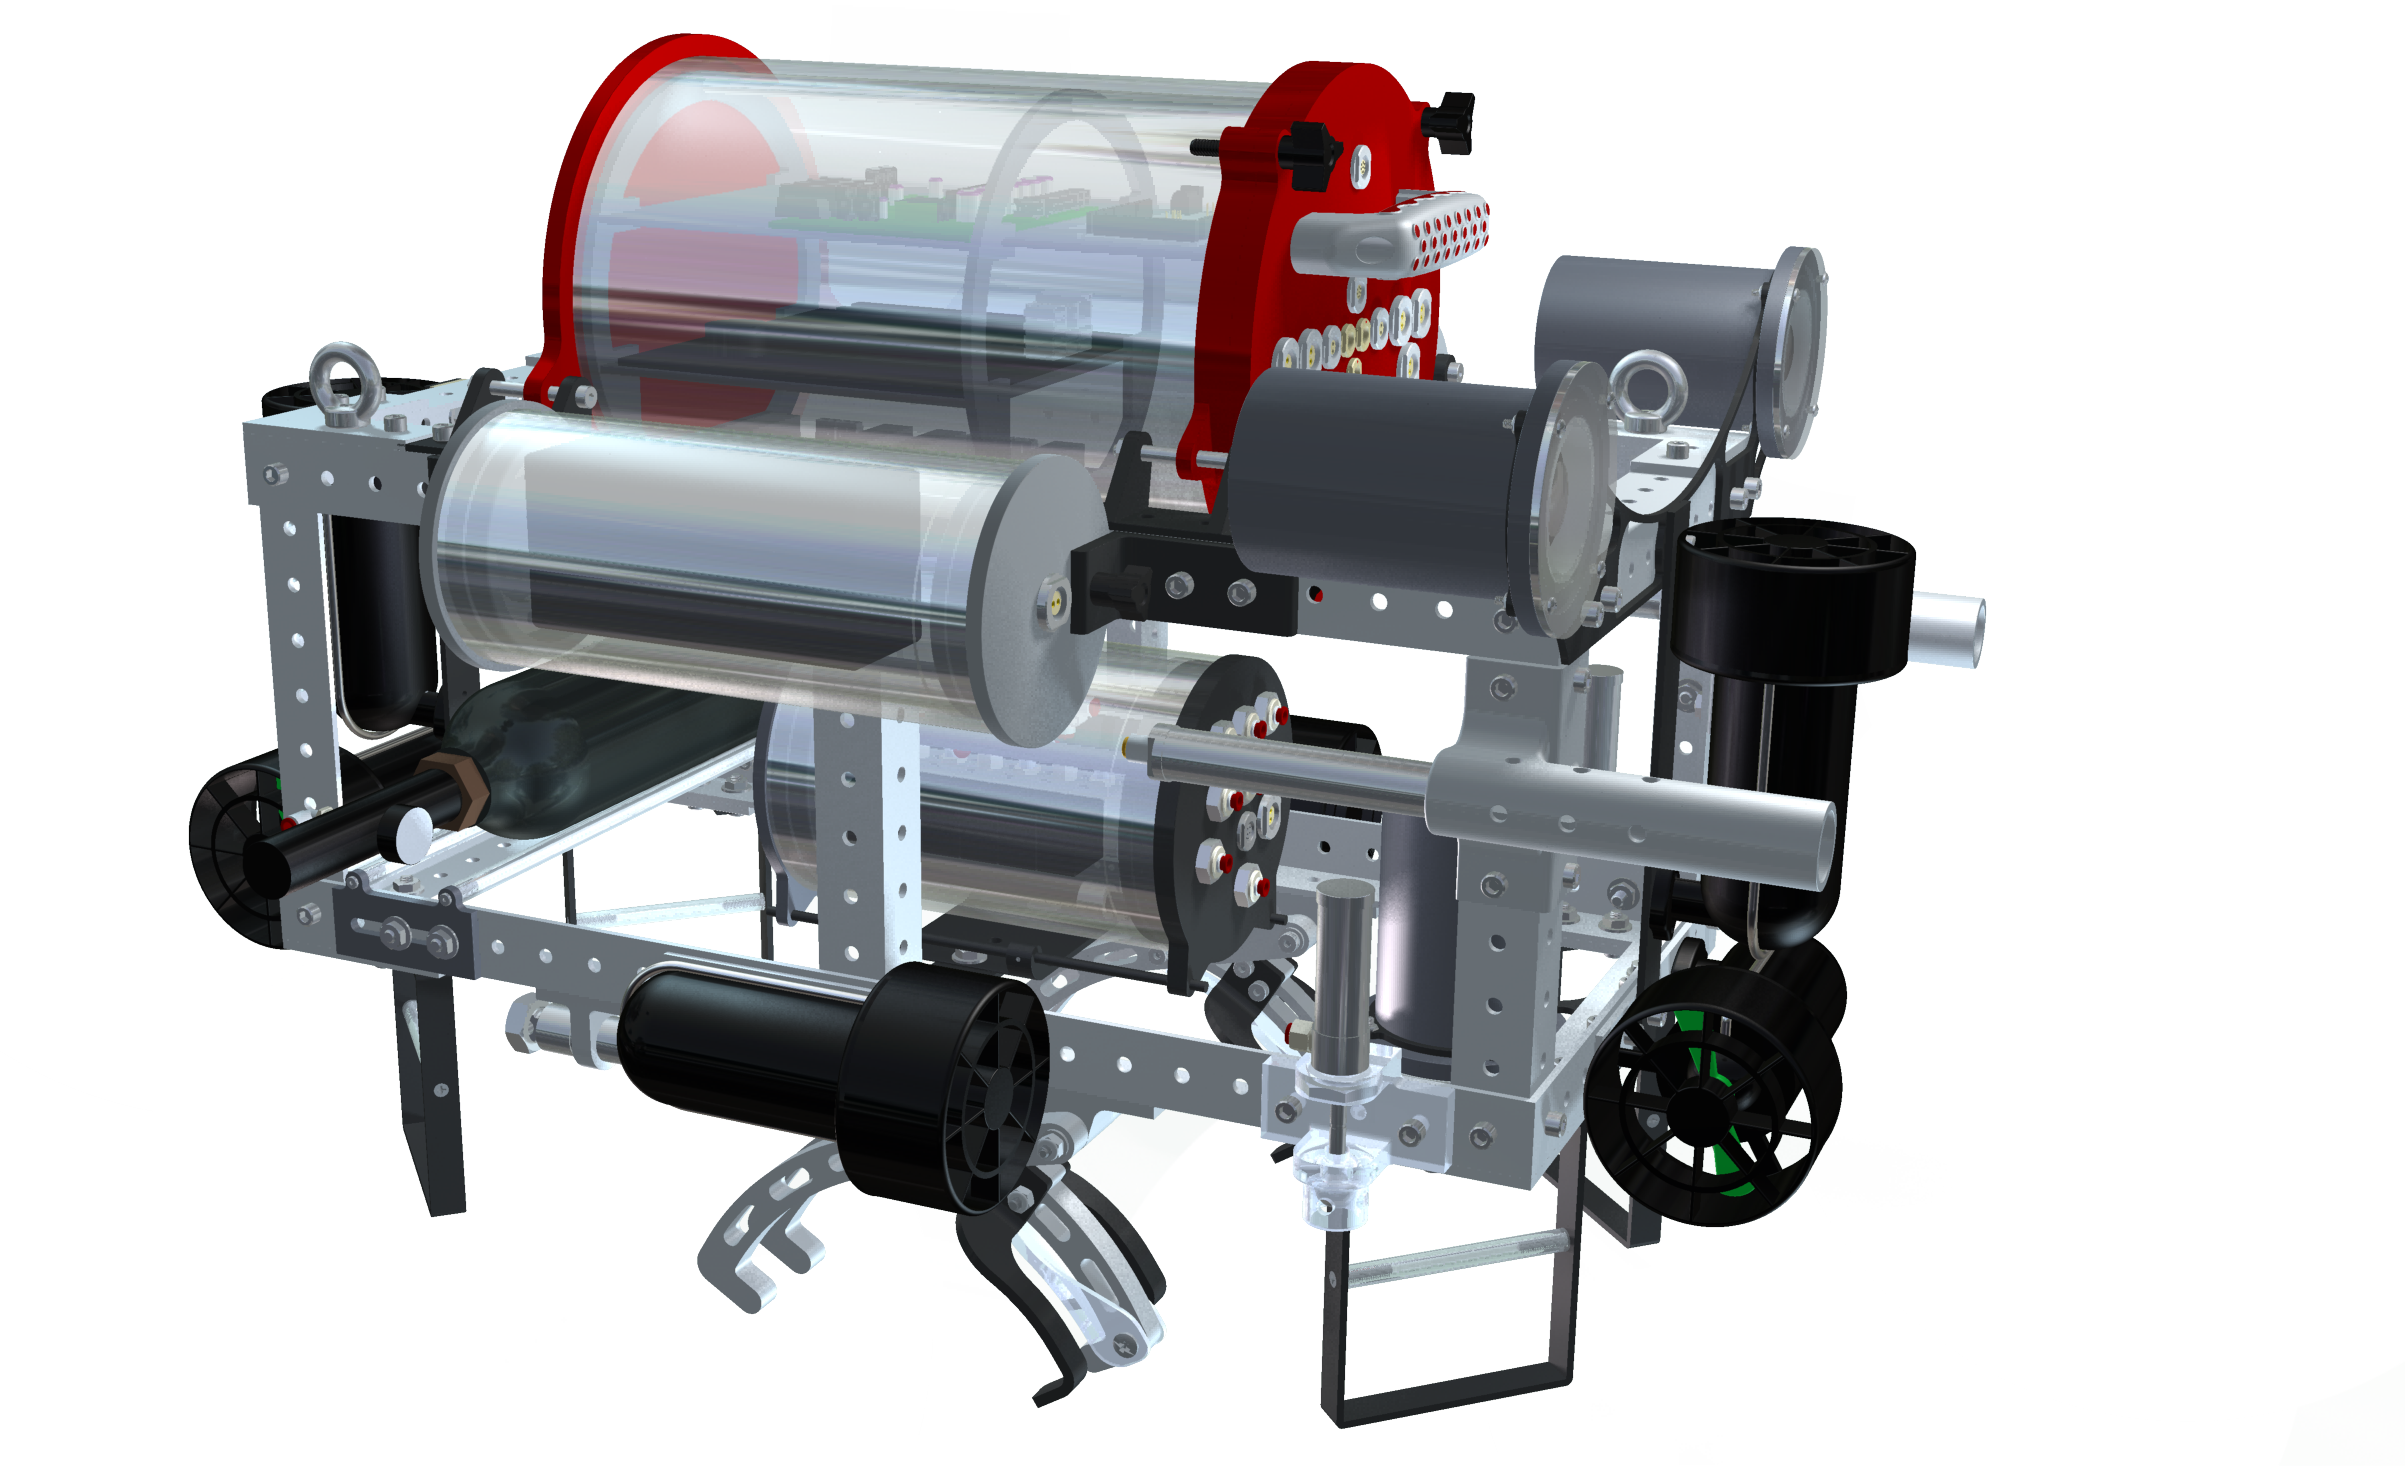
\includegraphics[height=4.2in]{media/full_assembly.png}
\caption{AUV assembly}
\label{auv_assembly}
\end{figure}

Figure~\ref{auv_assembly} shows the current CAD model of the entire AUV. It consists of a frame, a main hull pressure vessel, two battery pressure vessels, three camera pressure vessels, a pneumatic valve housing, an IMU pressure vessel, two claw mechanisms, two marker dropping devices, two pneumatic torpedoes, a $CO_2$ tank, and six thrusters.  The majority of the materials are HDPE plastic, 3D-printed resin, and aluminum.  All designs are from scratch, except for fasteners and electrical components. 
\end{samepage}


\begin{samepage}
\begin{figure}[H]
\centering
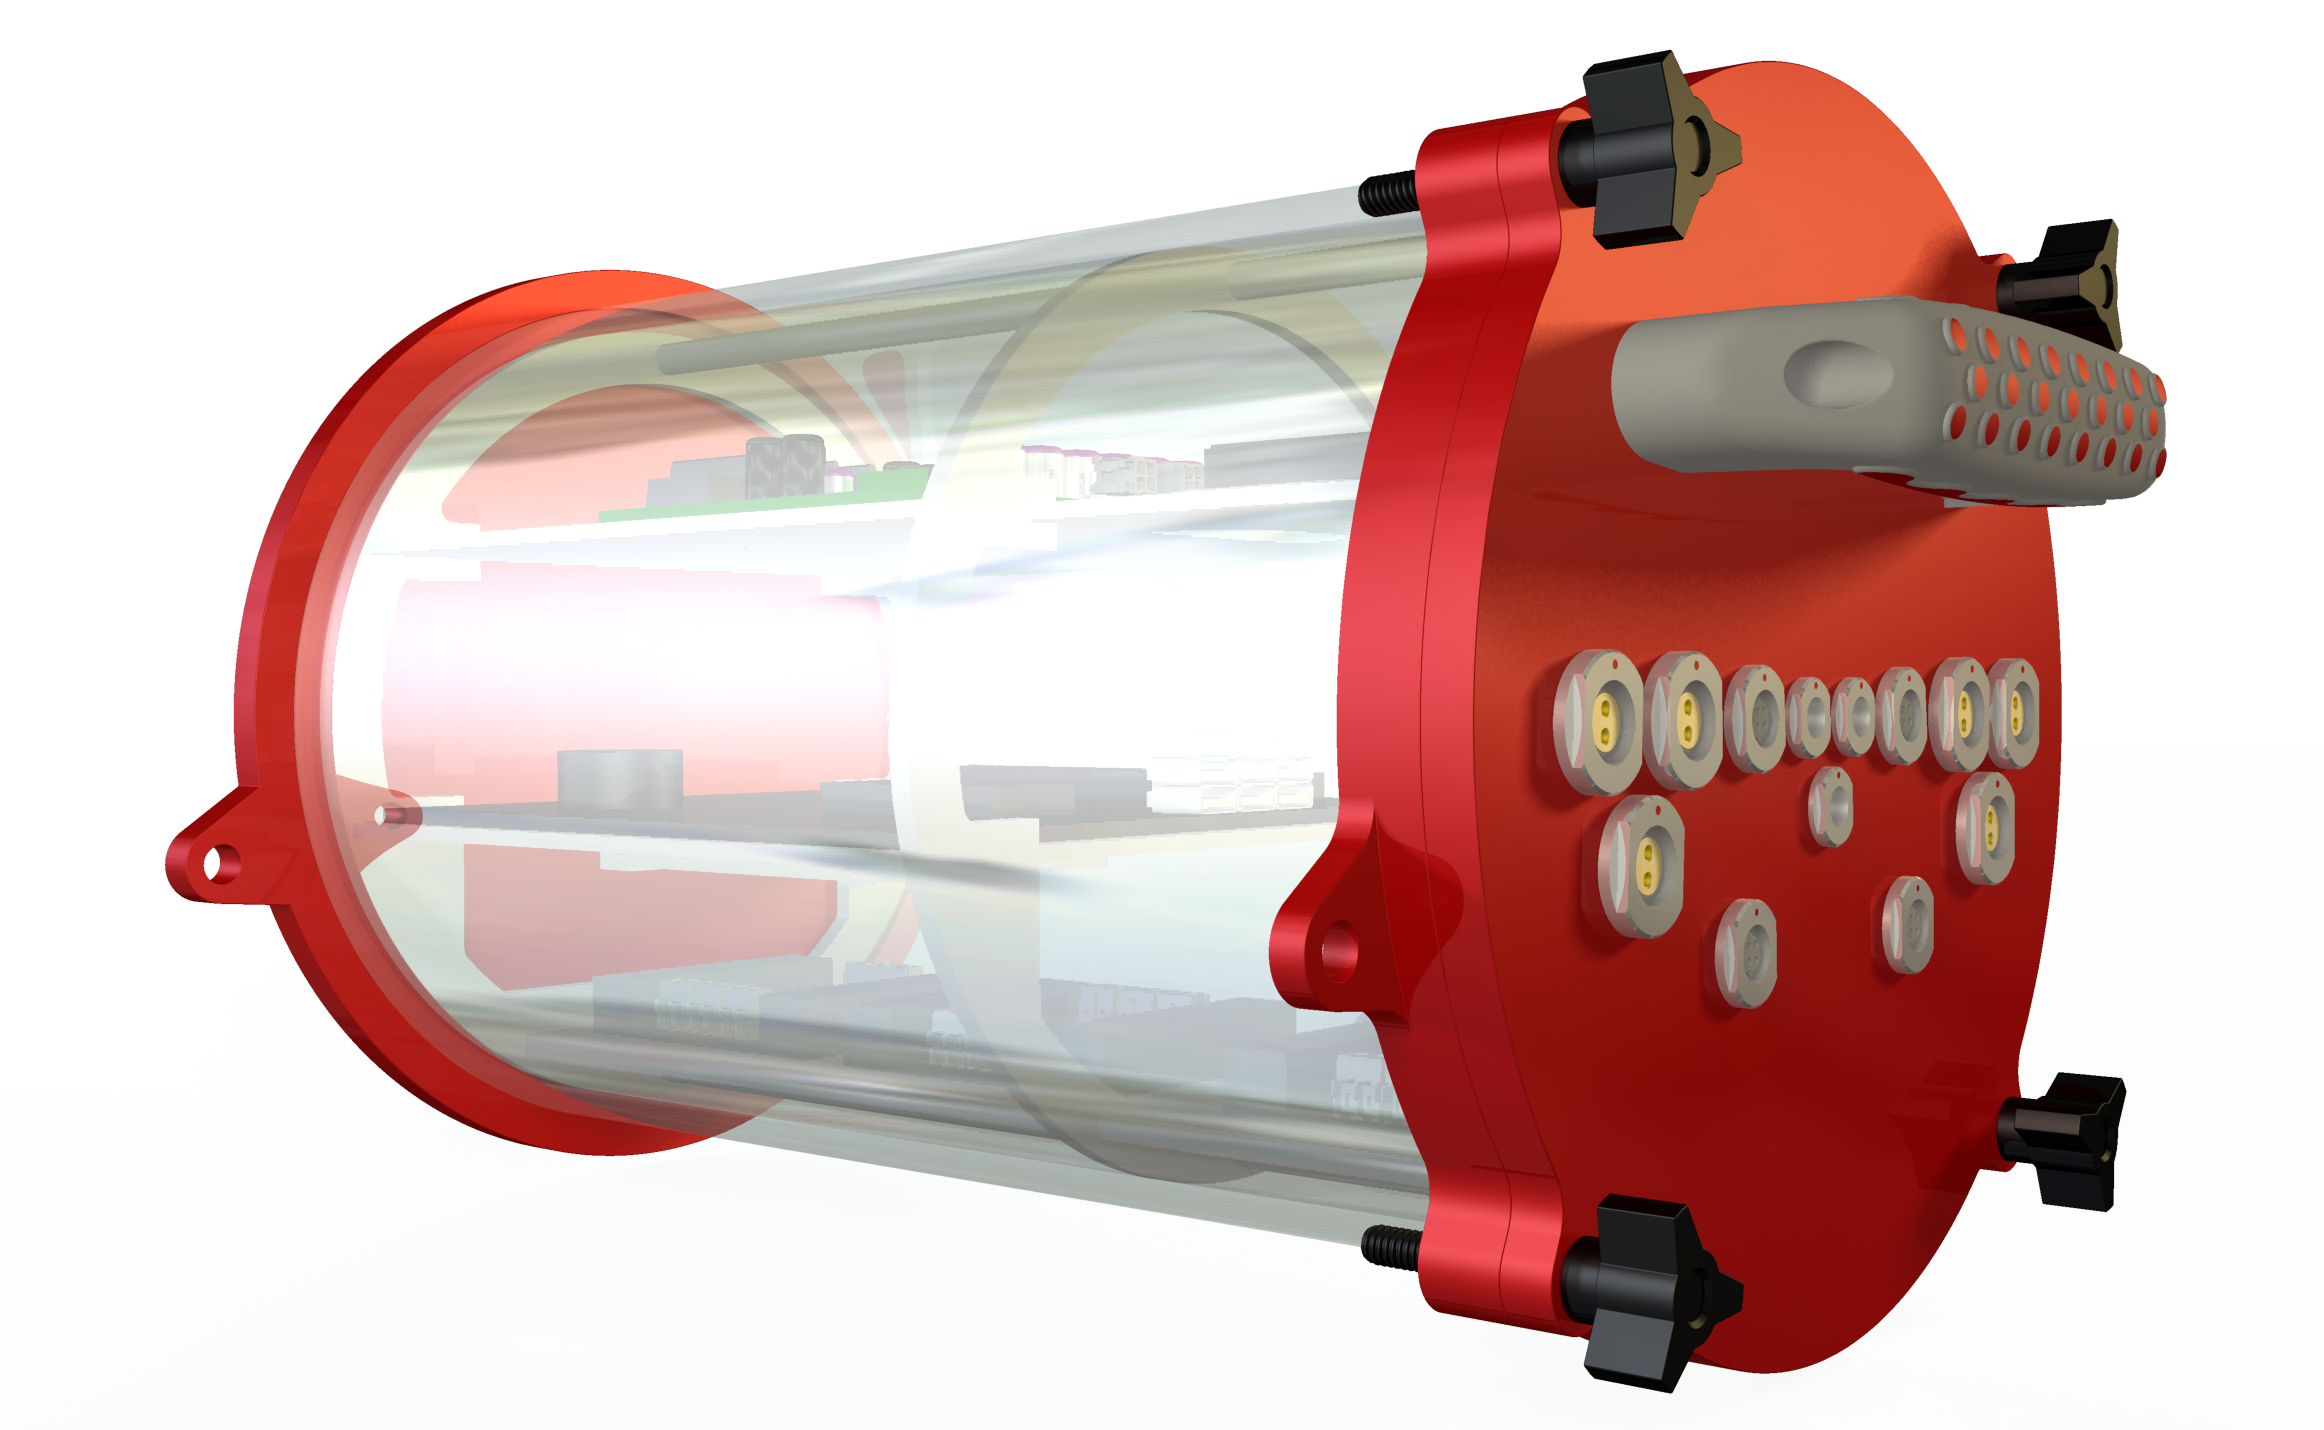
\includegraphics[height=4in]{media/main_hull.png}
\caption{Main hull pressure vessel}
\label{main_hull}
\end{figure}

The main hull houses most of the electronics and provides the majority of the buoyant force needed to keep the vehicle neutral and balanced. Inside, a rail system holds the electronics in place, and is removable from the front for easy access.  It attaches to the top of the frame, and connects all the electronic components using a set of waterproof connectors. 
\end{samepage}

\begin{figure}[H]
\centering
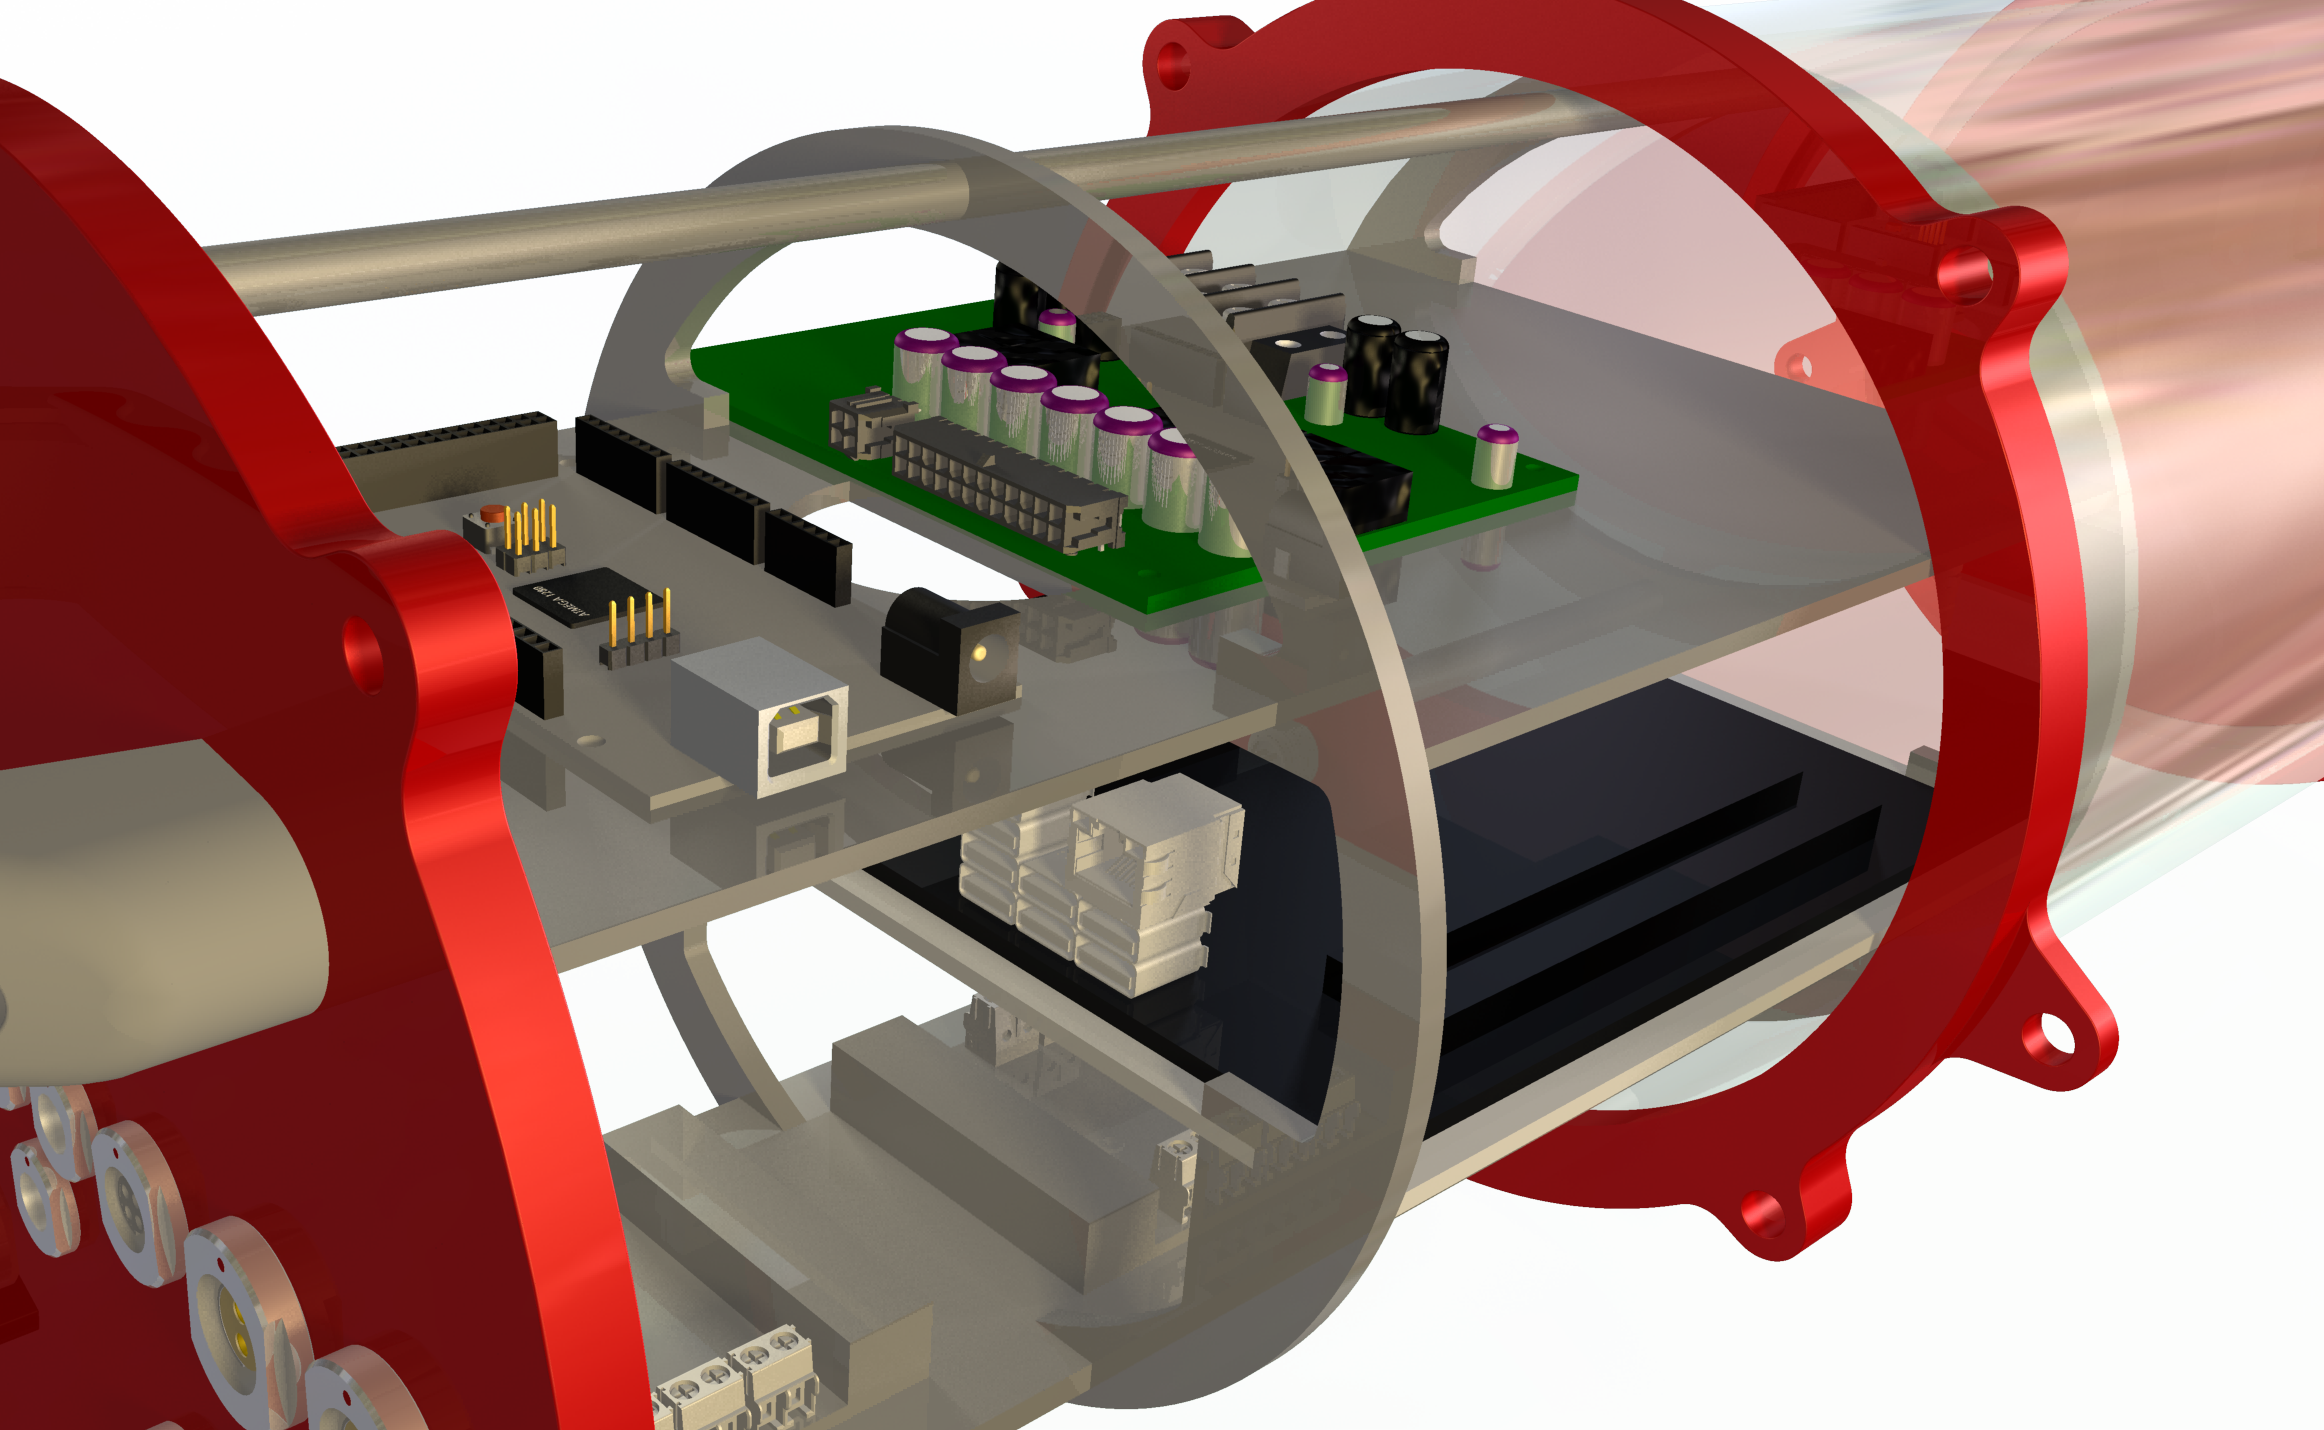
\includegraphics[height=4in]{media/MAIN-HULL-RENDER-2-ALPHA.png}
\caption{Internal electronics rack}
\label{main_hull2}
\end{figure}

Inside is the custom-built, on-board computer, as well as three motor controllers, an Arduino Mega, and a custom-built power distribution PCB board.  These electronics are needed to manage the six thrusters, the sensor array, and the computer vision system.  The frame is made of aluminum rails, with plastic racks, and uses a face O-ring with four nuts and vacuum seal to keep it water-tight. 

\begin{figure}[H]
\centering
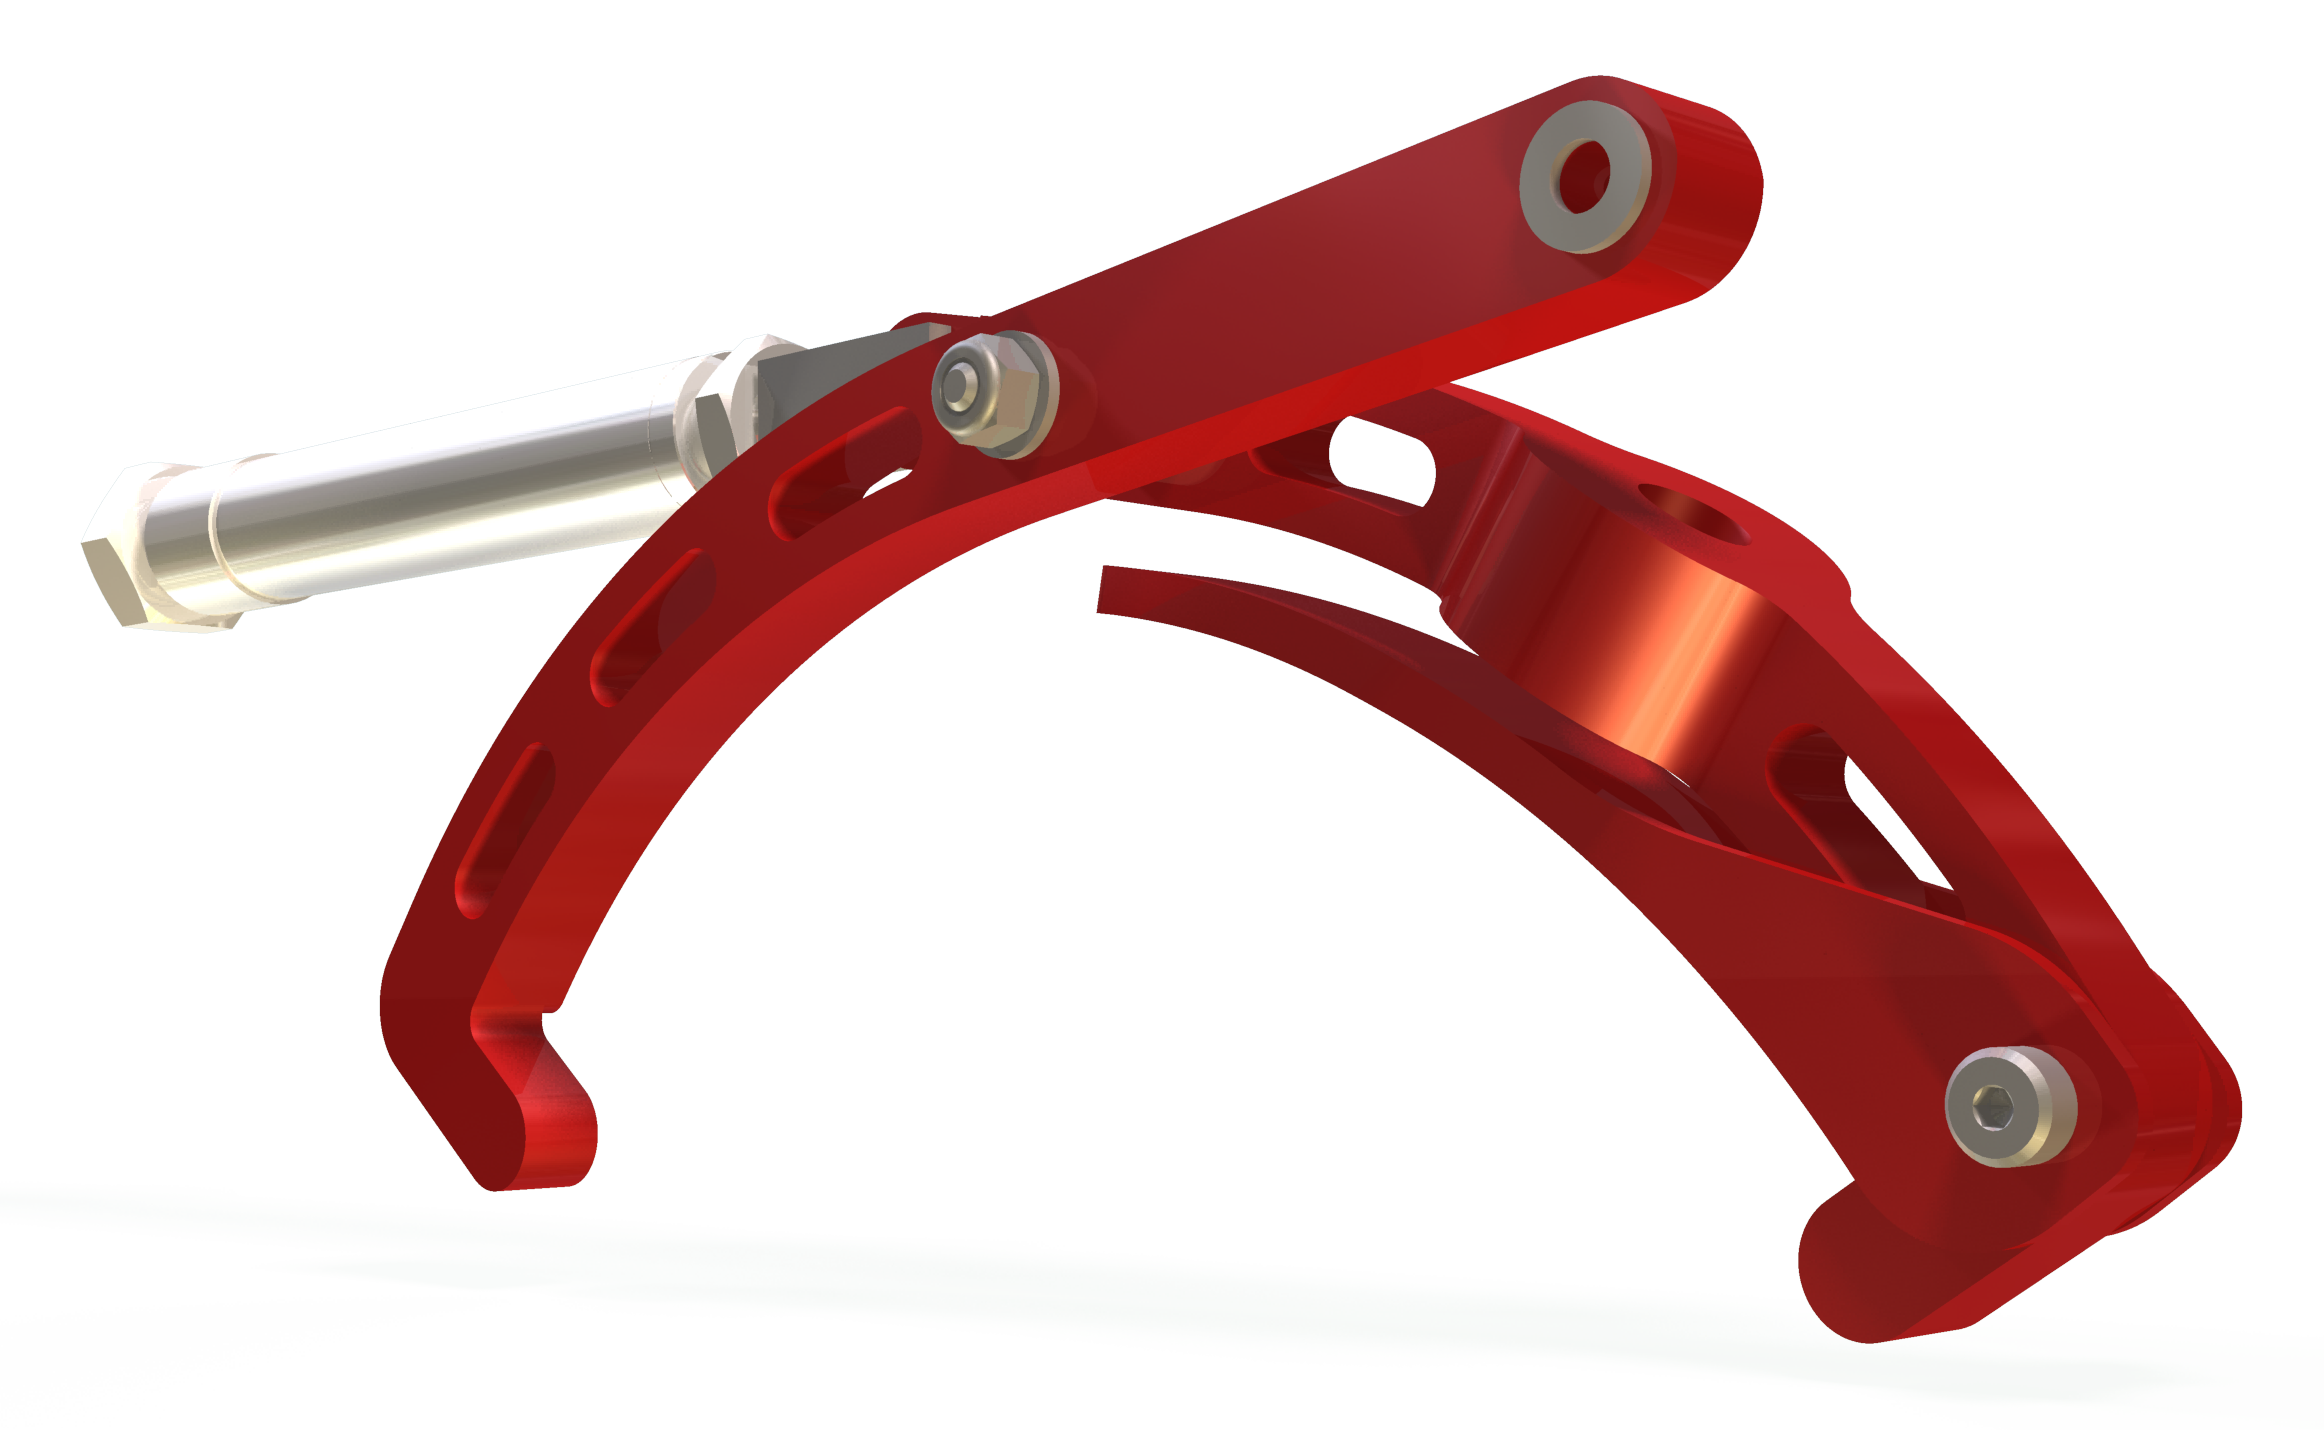
\includegraphics[height=4in]{media/GRABBER-RENDER-ALPHA.png}
\caption{Pneumatic claw device for picking up objects underwater}
\label{grabber}
\end{figure}

The pneumatic claw uses a double-acting piston to open and close two ``fingers'' of the claw, which are printed in an Stratasys Objet260 3D printer.  A lever on one of the fingers senses when an object has successfully been picked up using a custom, waterproof limit switch.  

\begin{figure}[H]
\centering
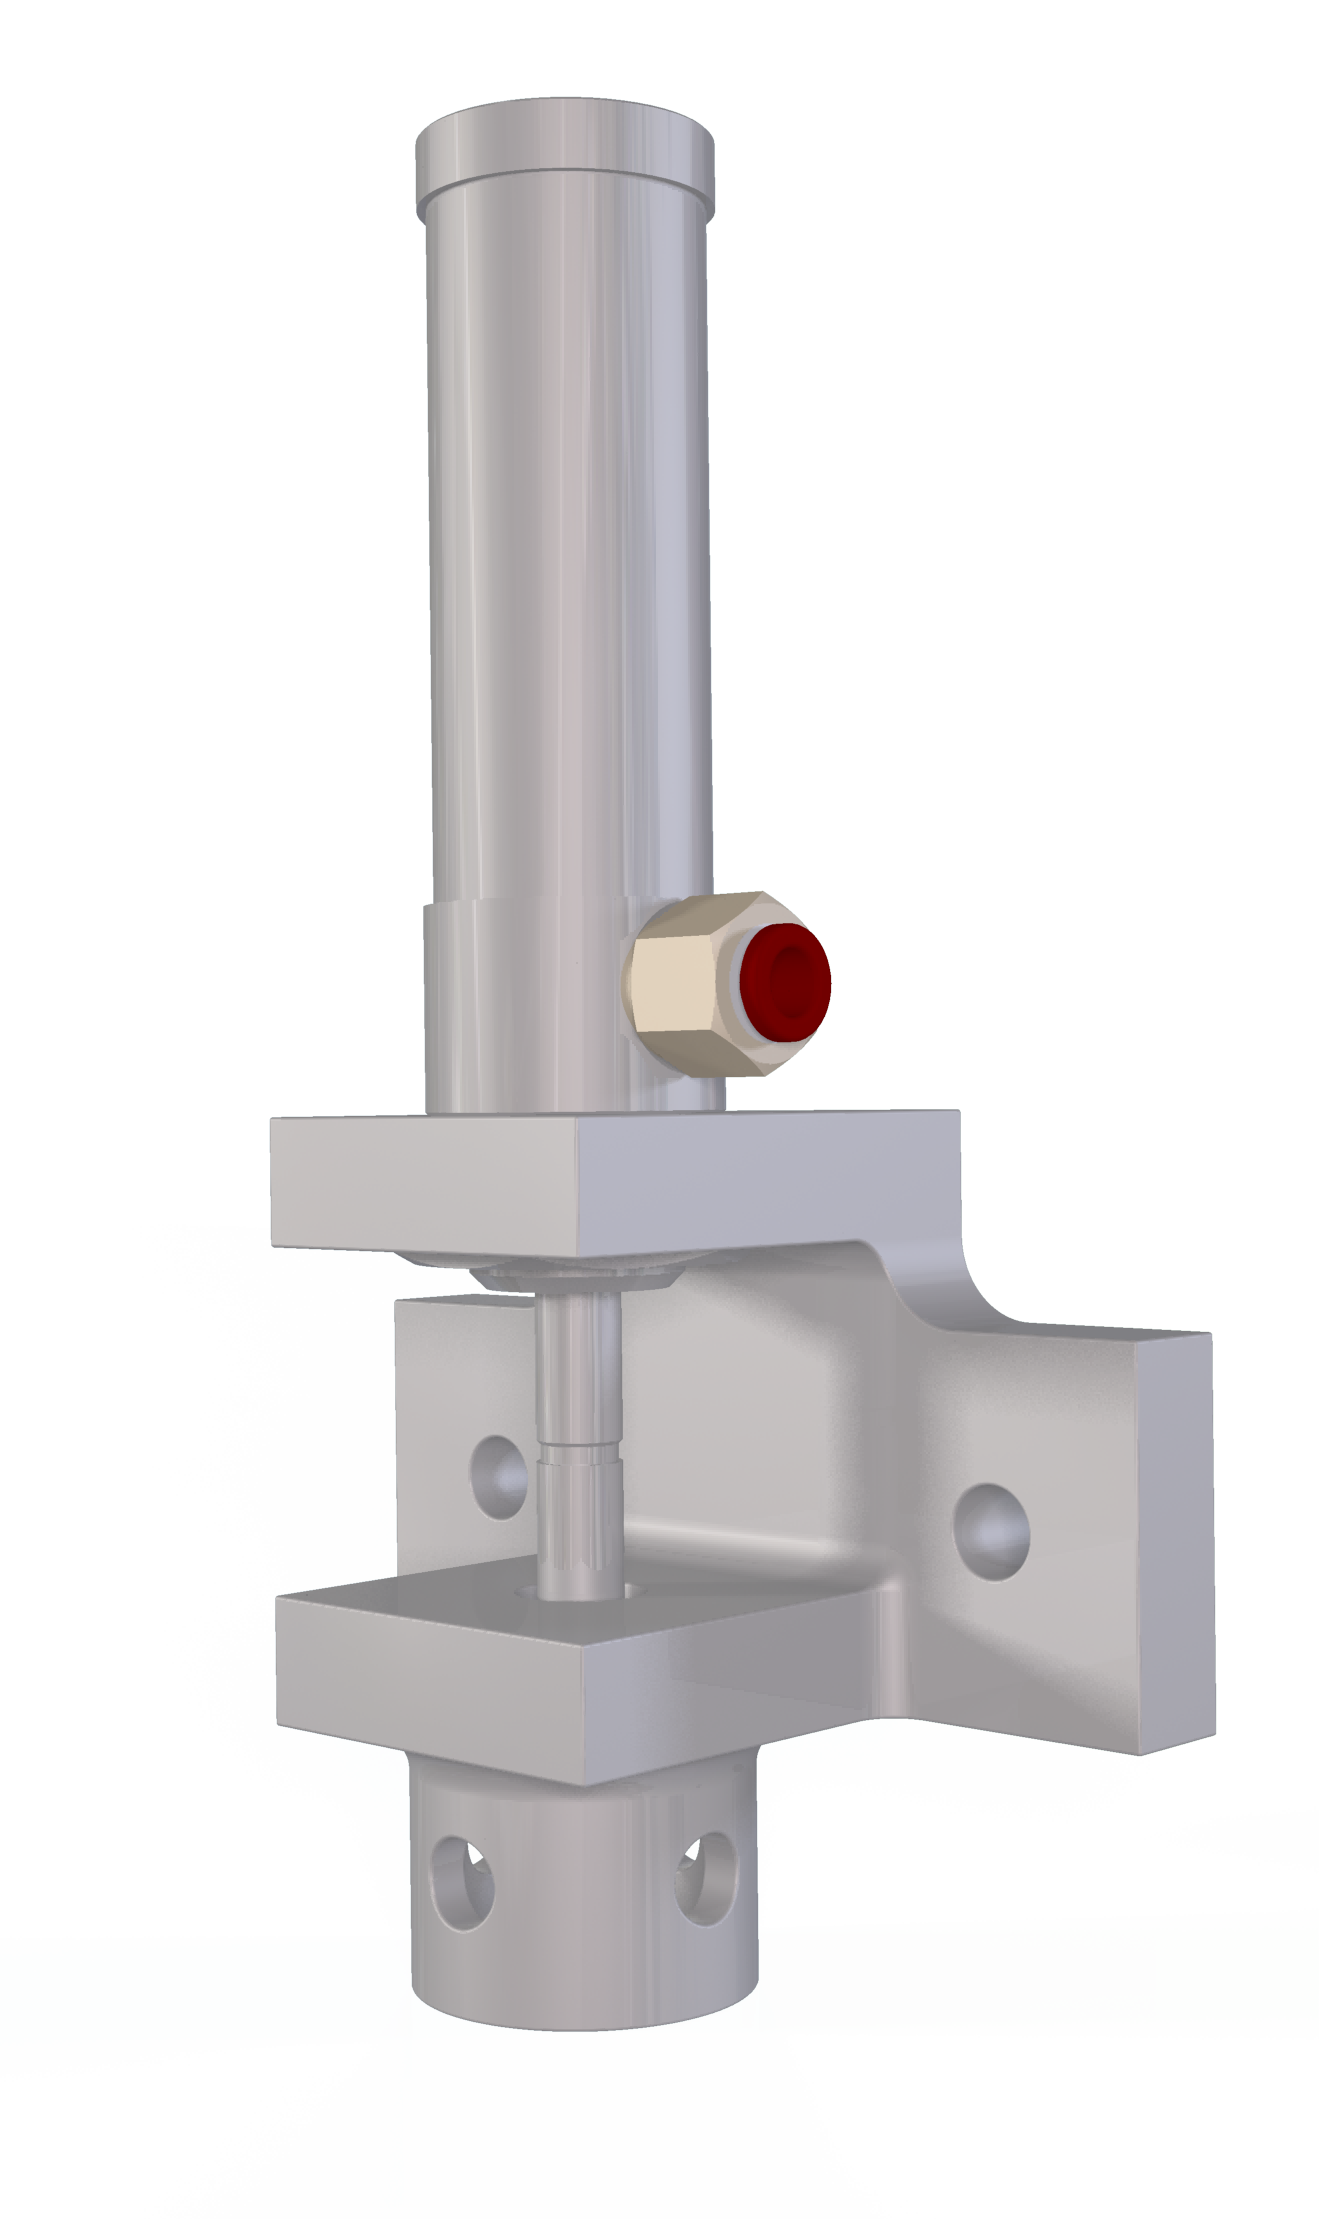
\includegraphics[height=4in]{media/marker_dropper.png}
\caption{Pneumatic marker dropper device}
\label{marker}
\end{figure}

The pneumatic marker dropper uses a reverse-acting piston with a magnet to release a ball bearing marker when over a target.  It is printed in a FormLabs Form 1 3D printer and coated with a protective sealant.

\begin{figure}[H]
\centering
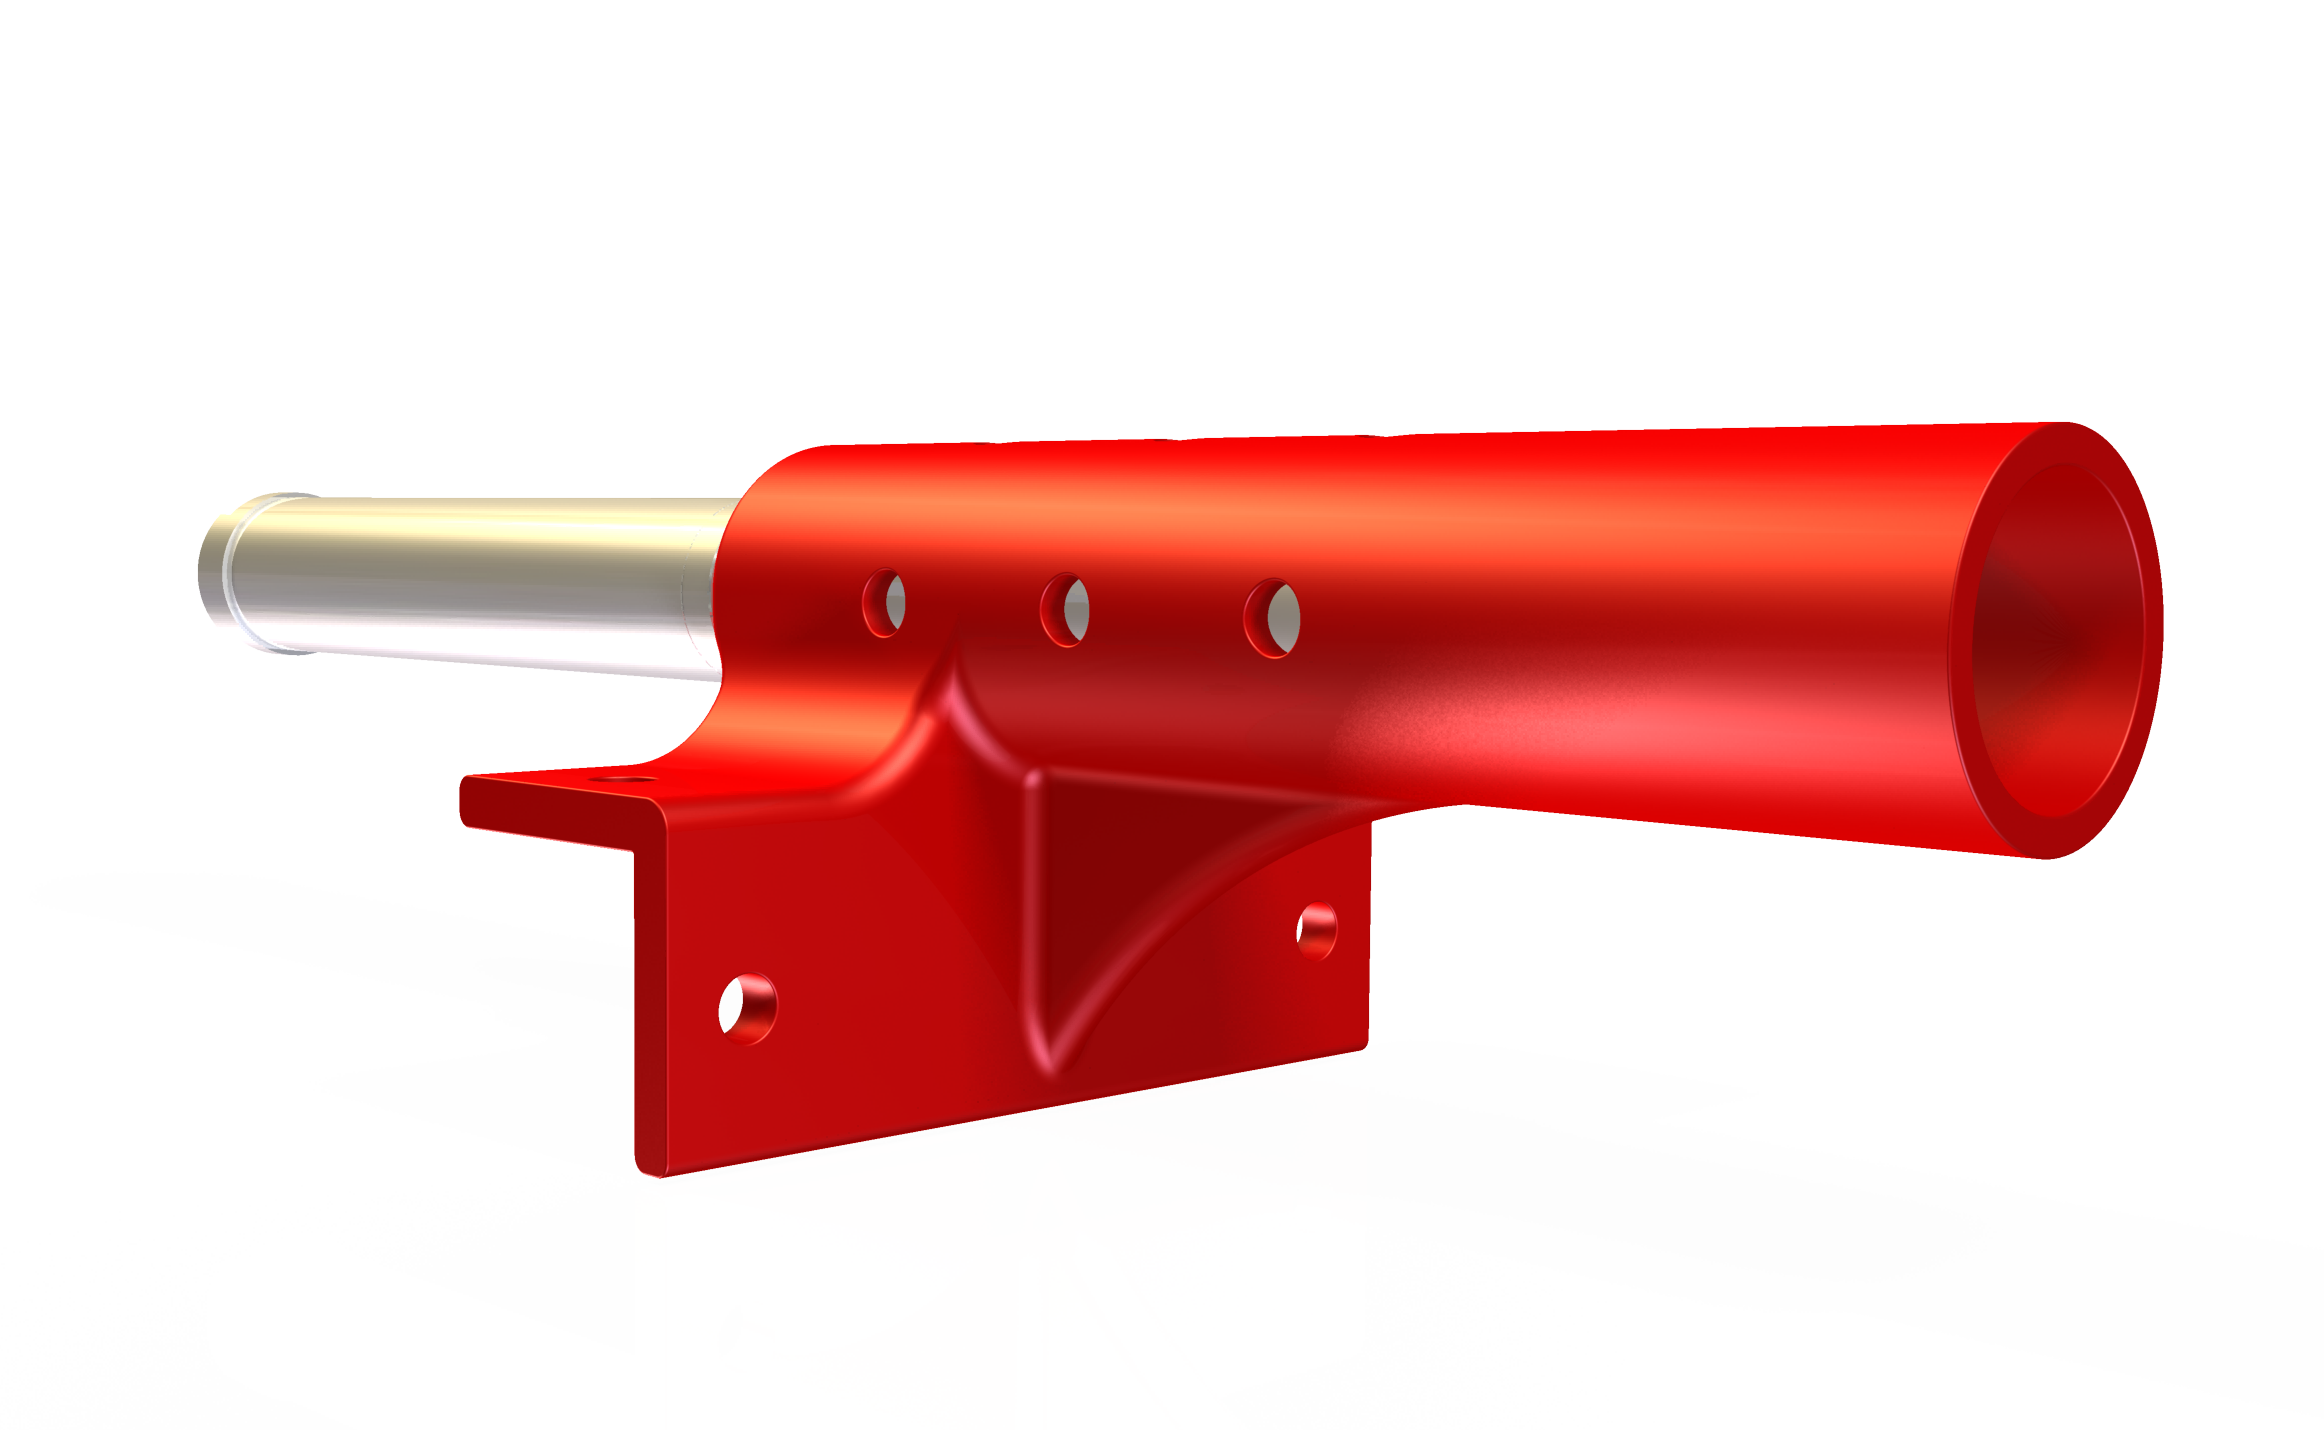
\includegraphics[height=4in]{media/TORPEDO-RENDER-ALPHA.png}
\caption{Pneumatic torpedo launcher}
\label{torpedo}
\end{figure}

The torpedo launcher uses a pneumatic piston to fire a custom, 3D-printed projectile at a target at a distance of up to 5 meters.  It is printed in a FormLabs Form 1 3D printer and coated with a protective sealant.

\begin{figure}[H]
\centering
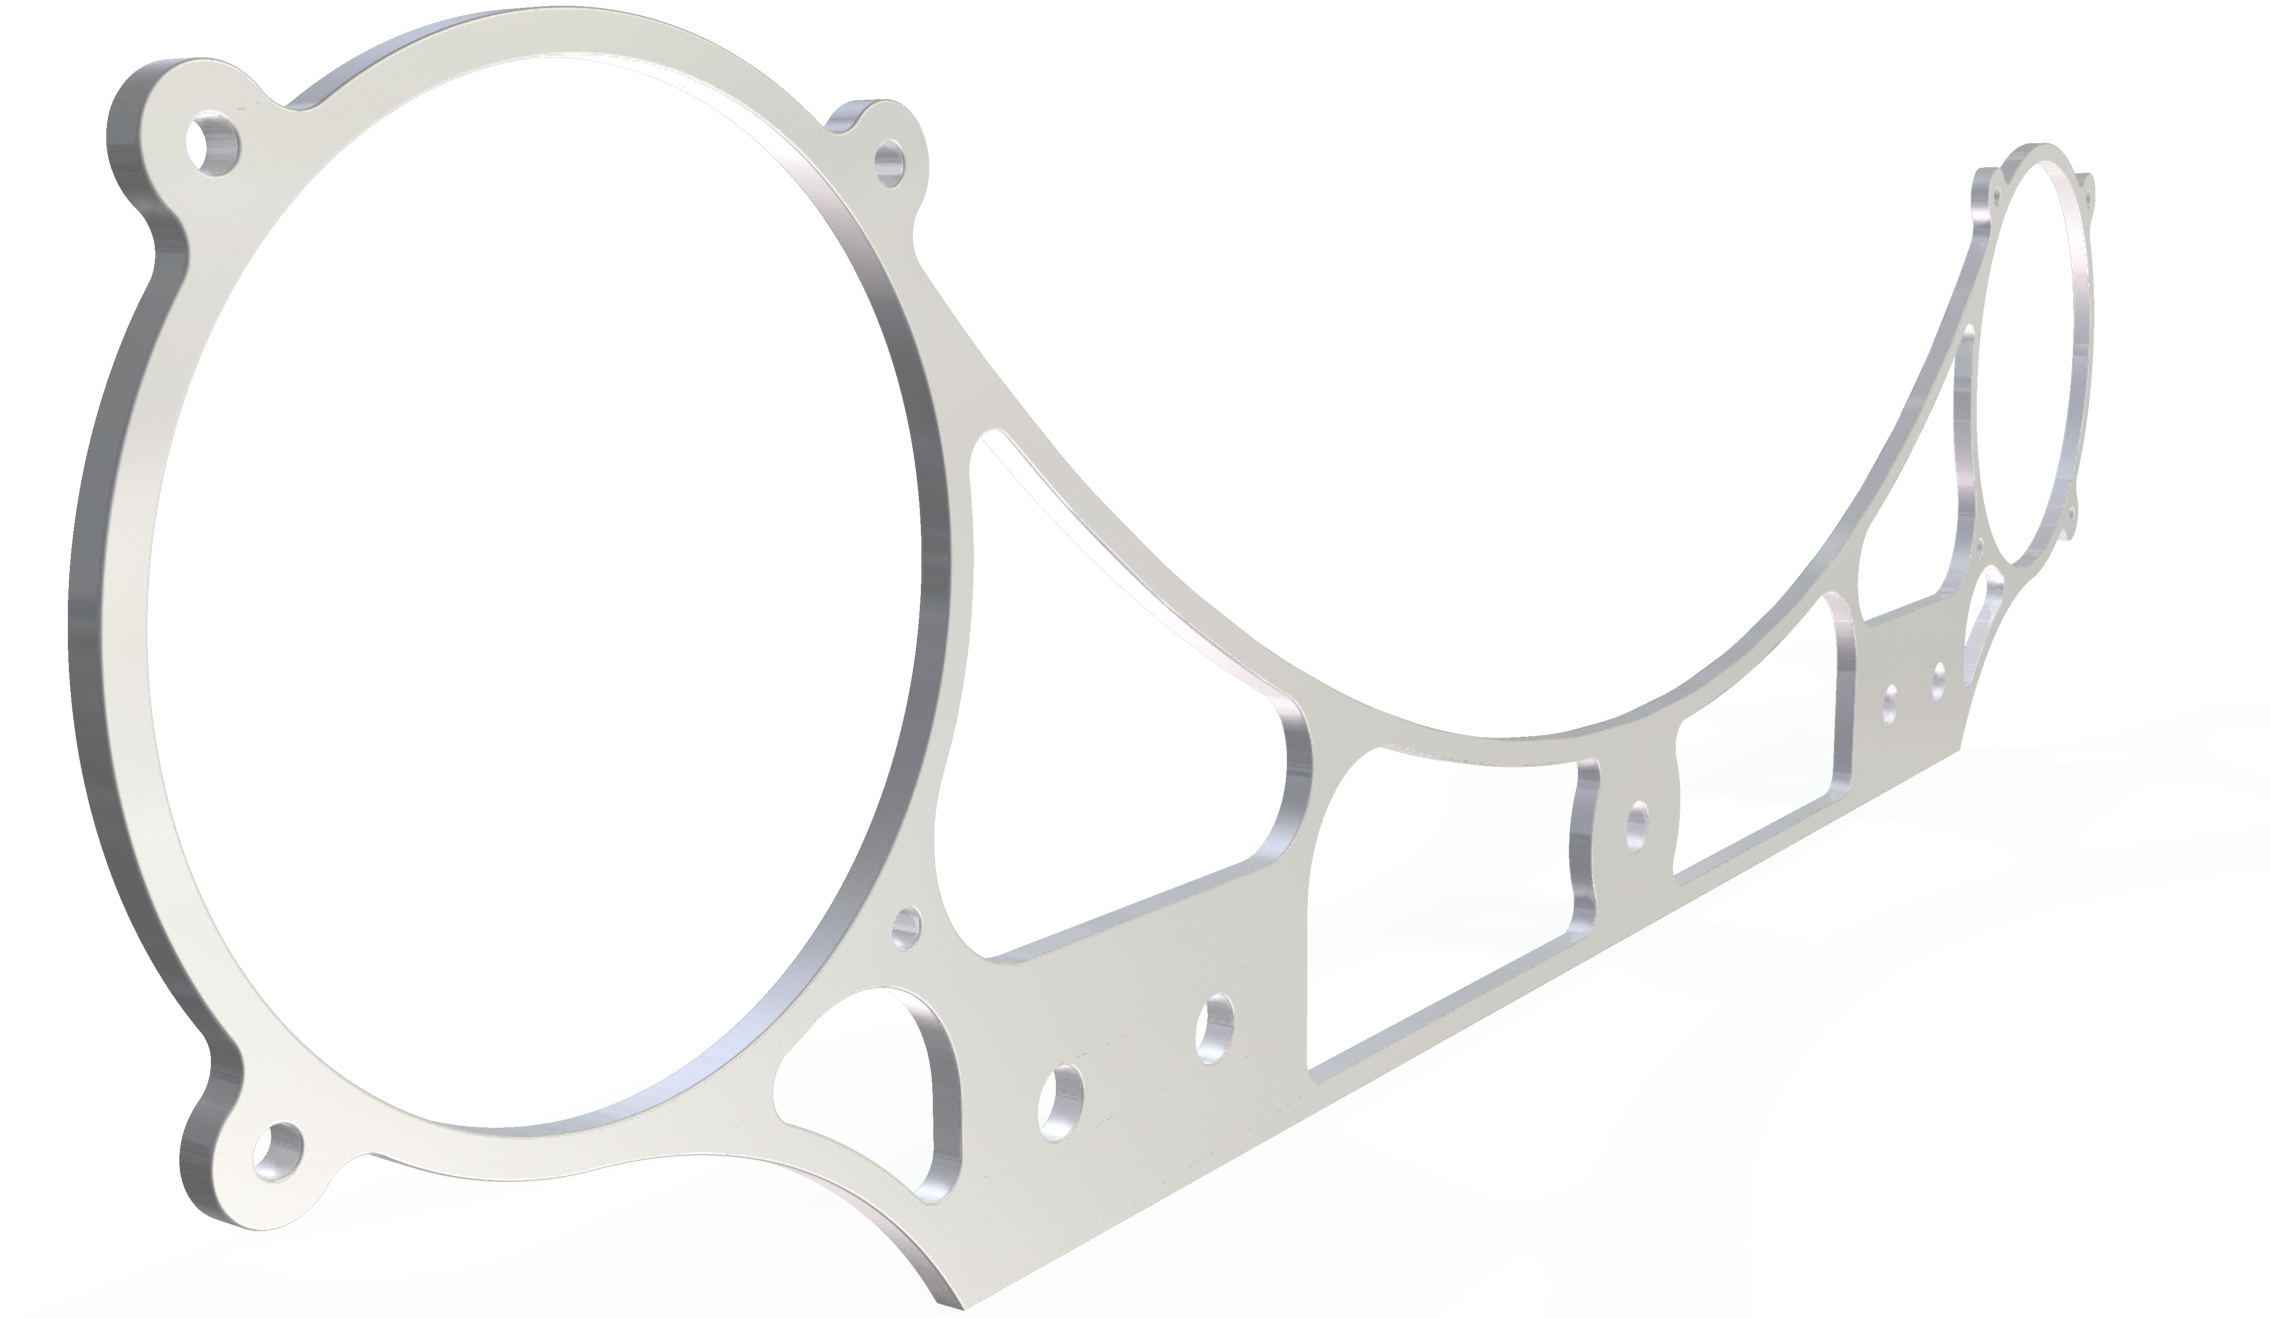
\includegraphics[height=4in]{media/front_camera_bracket.png}
\caption{Front-facing CNCed camera bracket}
\label{camera_bracket}
\end{figure}

The front-facing camera bracket connects two cameras to the bow to allow for stereo vision.  The bracket is CNCed from a sheet of aluminum for rigidity and shaped to maximize the distance between the cameras and reduce weight.  Like all the machined aluminum parts, it will be anodized following machining to prevent corrosion.

\begin{figure}[H]
\centering
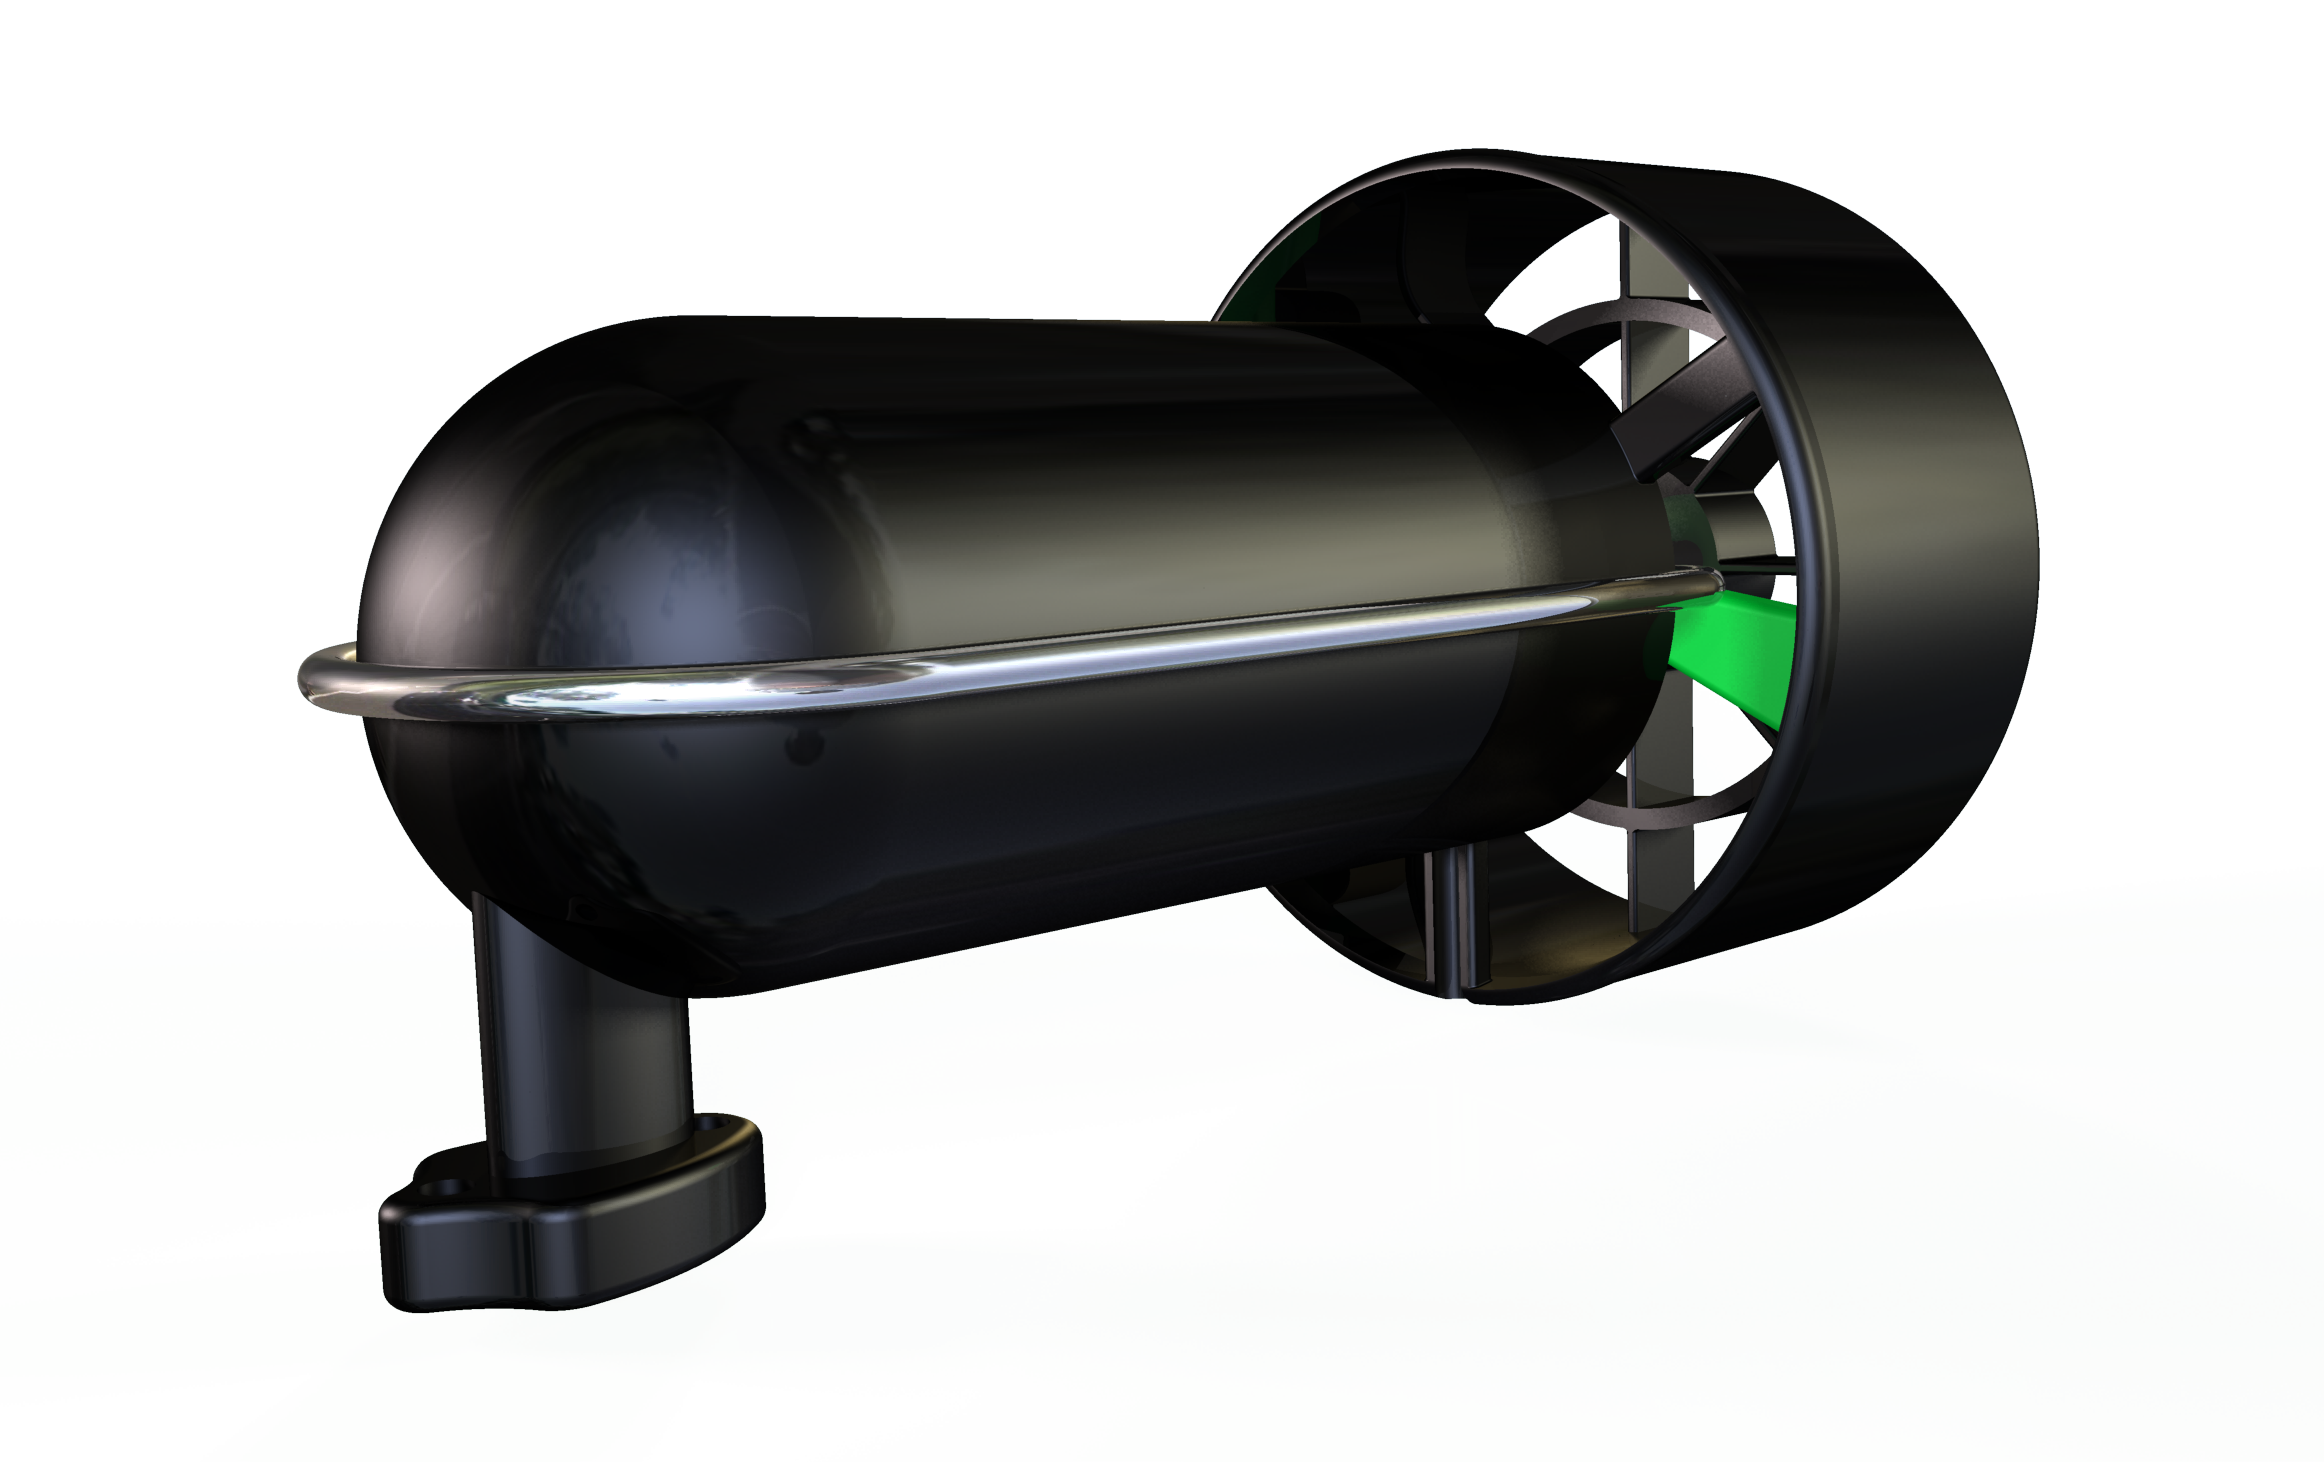
\includegraphics[height=4in]{media/THRUSTER-RENDER-2-ALPHA.png}
\caption{CAD model of the Seabotix BTD150 thruster}
\label{thruster}
\end{figure}

Six Seabotix BTD150 thrusters drive the vehicle and are arranged for five degrees of freedom - active surge, sway, heave, yaw, and pitch.

\clearpage

\section{Variable-friction Shoe Mechanism}
\paragraph{Project:} Research project for Professor~\href{http://www.cim.mcgill.ca/~jer/}{Jeremy Cooperstock} of~ \href{http://www.cim.mcgill.ca/sre}{The Shared Reality Lab} - McGill Centre for Intelligent Machines
\paragraph{Goal:} Design, manufacture, assemble and demonstrate a mechanism to fit in a shoe that can control the coefficient of friction between the shoe and the floor surface.
\paragraph{Process:}  Based on research done by Guillaume Millet, Martin Otis, and Jeremy Cooperstock into various methods of varying friction during natural walking and the applications for this type of simulated environment, a concept is created in one semester.  This involves choosing a method of deployment, researching all components and materials, calculating needed geometry and movements, designing the layout, and analyzing the stresses.  The next semester is for manufacturing, assembling and testing the apparatus. This involves ordering materials and parts, machining and assembling components, developing the power and control system, and testing the mechanism prototype.  

The full design report of the concept can be found at~\href{http://michaelelliotking.com/report}{michaelelliotking.com/report}.

\begin{figure}[H]
\centering
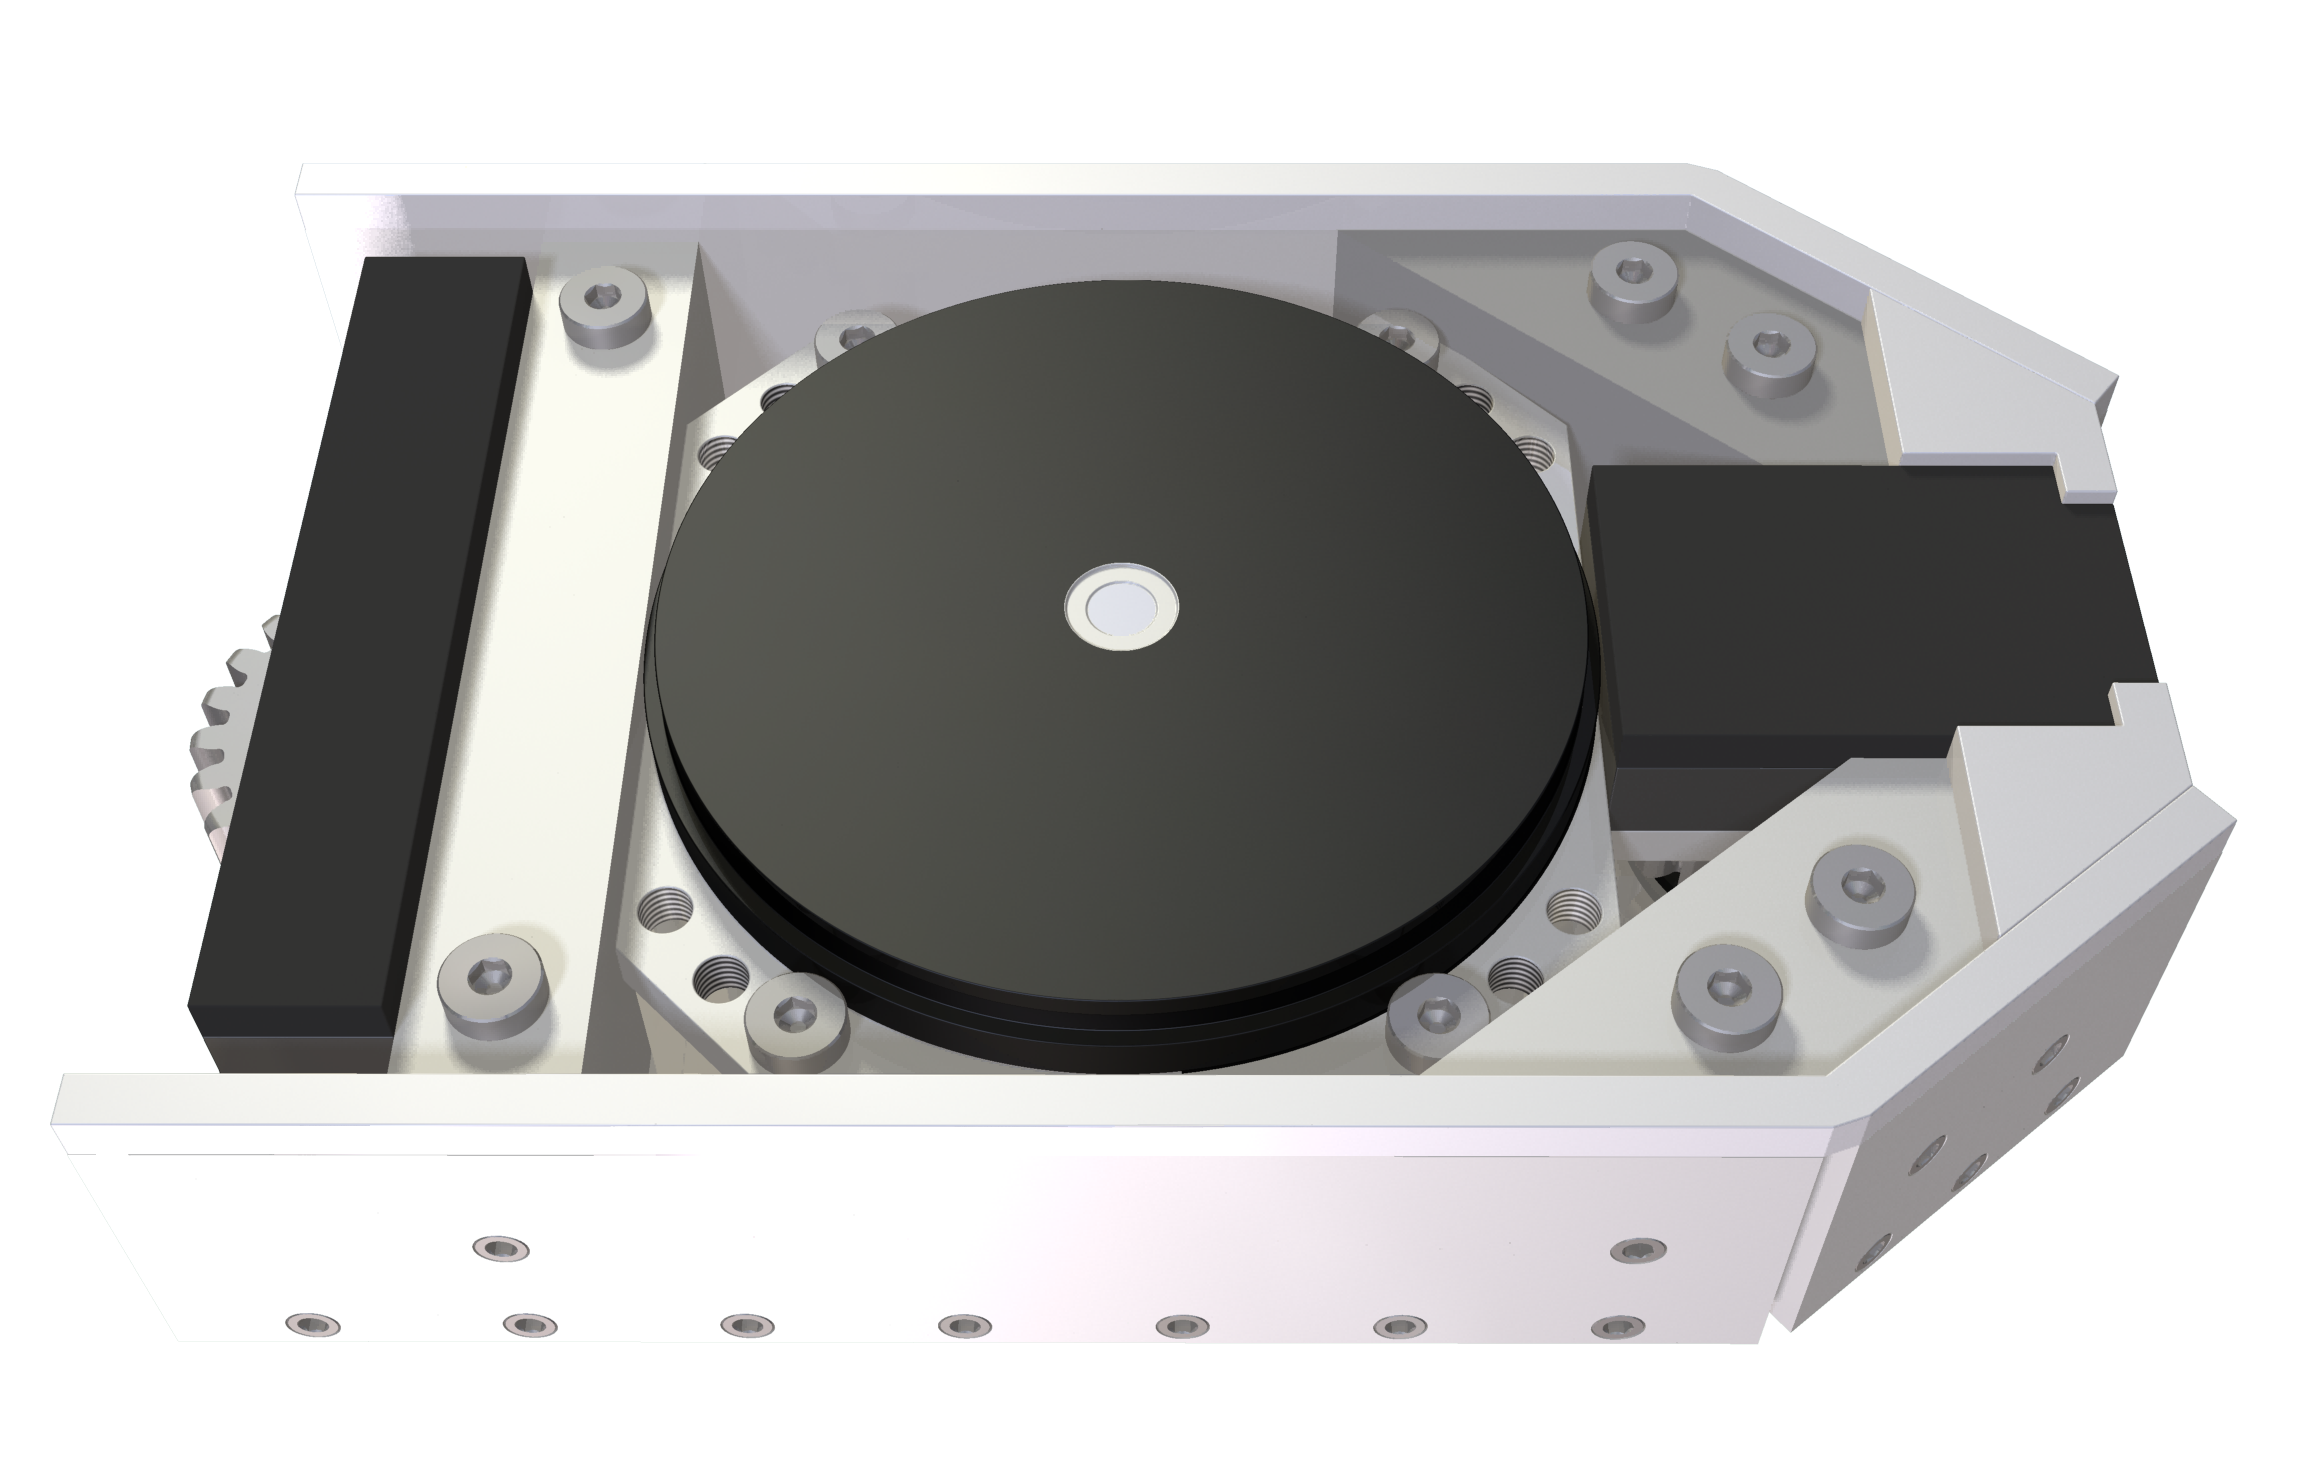
\includegraphics[height=4in]{media/side_overview.png}
\caption{Assembly of the variable-friction shoe mechanism}
\label{overview}
\end{figure}

The variable-friction shoe mechanism controls how much a high-friction material protrudes past a low-friction material to vary the friction force and simulate different surfaces. It uses two lead screw mechanisms, a gear train and a stepper motor to extend two rubber-covered ``brakes'' past the outer strip of Teflon.

\begin{figure}[H]
\centering
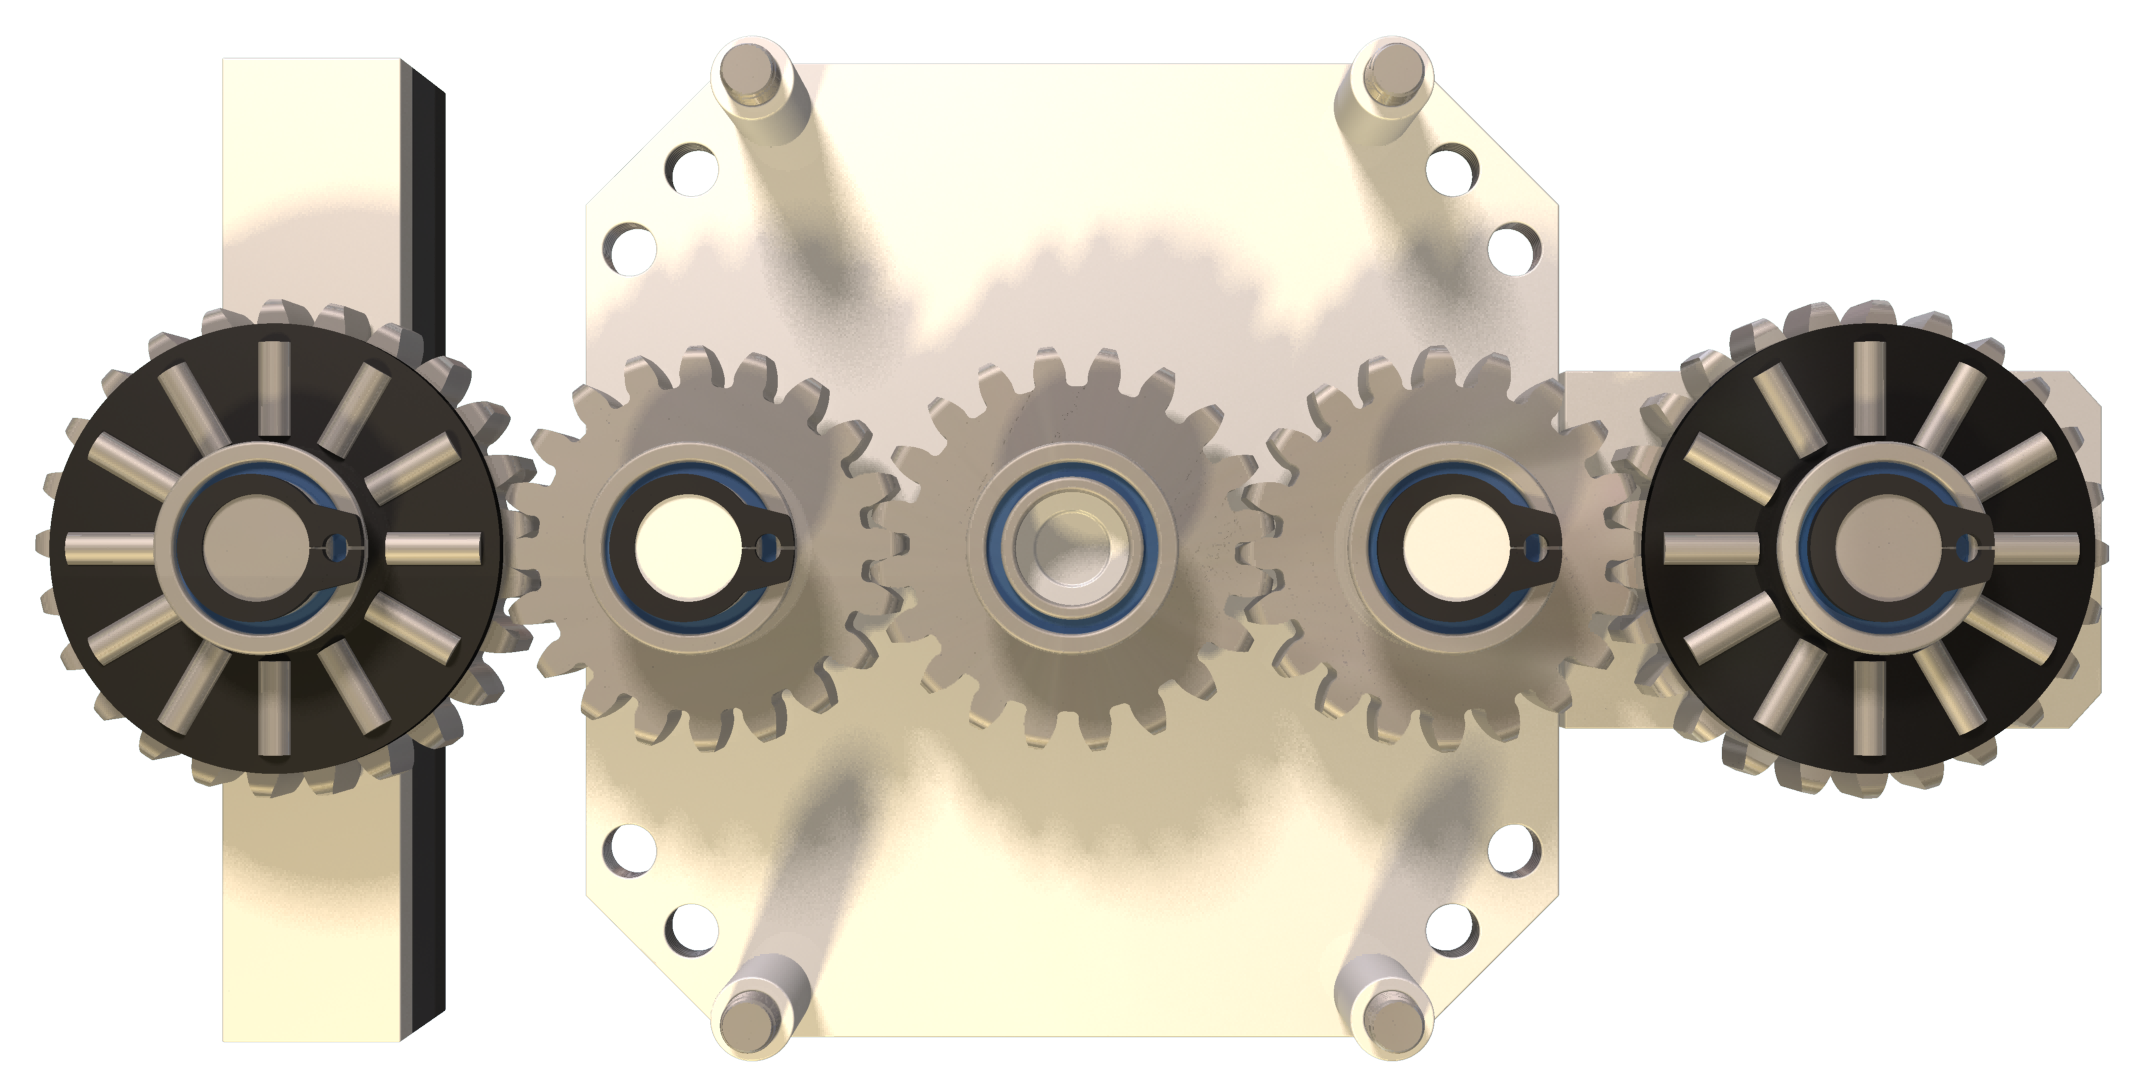
\includegraphics[height=4in]{media/bottom.png}
\caption{Bottom view of gear train and bearings}
\label{bottom}
\end{figure}

Figure~\ref{bottom} shows the gear train that translates the discrete rotations of the stepper motor to the outer gears, which are fixed to the lead screws that drive the brakes.  Also shown are the ball bearings and needle roller bearings that support the moving parts while withstanding loads of a walking person.

\begin{figure}[H]
\centering
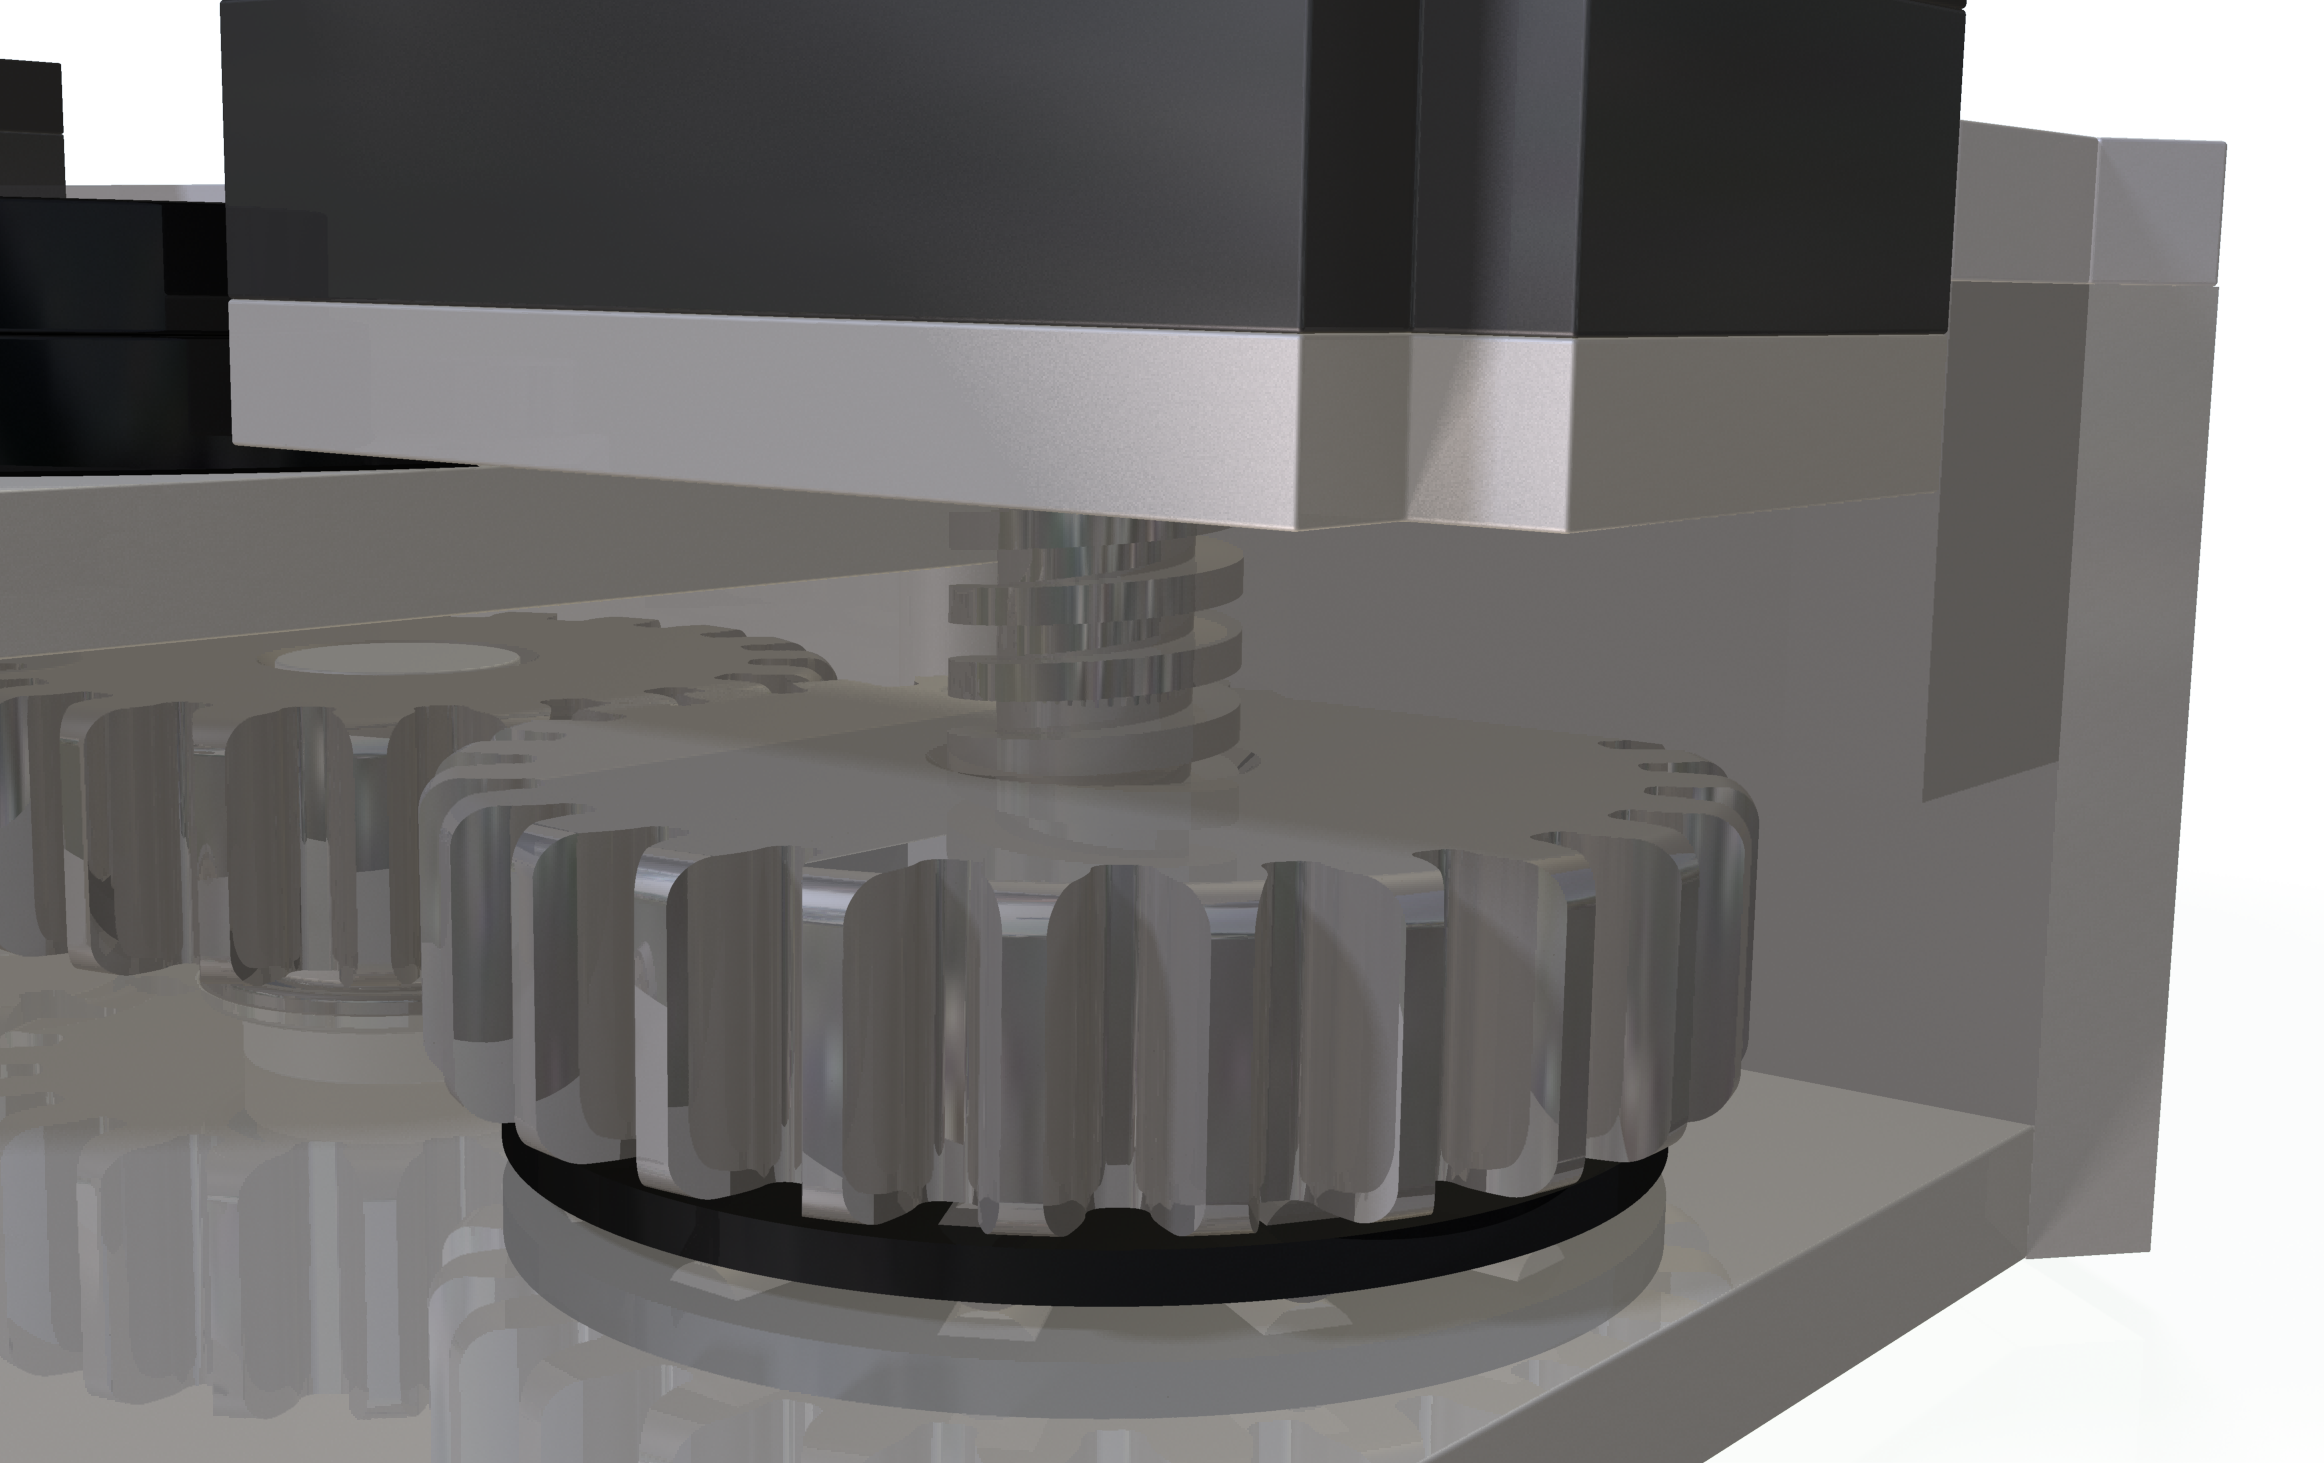
\includegraphics[height=4in]{media/back_brake_close.png}
\caption{Cut-away view of gear, lead screw and brake}
\label{brake}
\end{figure}

The lead screw is press-fitted to the gear and threaded into the aluminum plate of the brake.  The brake consists of a metal plate, a piece of EVA foam for elasticity, and a strip of rubber for high-friction.  The brake system allows for precise translations as small as a tenth of a millimeter, which is needed to achieve specific coefficients of friction.

\clearpage

\section{}
{\LARGE For the sake of time, I have only included my most recent work.  I will continue to update this portfolio with my work - both old and new - and it will continue to be available at \href{http://www/michaelelliotking.com/portfolio}{www.michaelelliotking.com/portfolio}.}\\[20pt]

\textbf{To be posted:}
\begin{itemize}
\item Material collection system for an autonomous lunar mining robot
\item Flying yacht conceptual design
\item Commercial aircraft wing design
\end{itemize}

\end{document}